\documentclass{report}

\usepackage{amsmath}
\usepackage{amssymb}
\usepackage{url}
\usepackage{float}

\usepackage{algpseudocode}
\usepackage{algorithm}

\usepackage{graphicx}
\graphicspath{ {images/} }

\addtolength{\oddsidemargin}{-.875in}
\addtolength{\evensidemargin}{-.875in}
\addtolength{\textwidth}{1.75in}

\addtolength{\topmargin}{-.875in}
\addtolength{\textheight}{1.75in}

\renewcommand{\vec}[1]{\mathbf{#1}}

\title{Hopp3r: a Planar 3 Degree of Freedom Hopping Robot}

\author{
Alex Friedman\\
Zen Iwankiw\\
Dan Lynch\\
Greg Niederschulte\\
Andrew SaLoutos\\
Suhail Pallath Sulaiman\\
Zidong Xiao\\
}

\begin{document}
%\maketitle

\begin{titlepage}
    \centering
    \vfill
    {\bfseries\Large
        Hopp3r\\
        \vskip2cm
        A Planar 3 Degree of Freedom Hopping Robot\\
    }    
    \vfill
    \includegraphics[width=\linewidth]{Hopp3r.jpeg} % also works with logo.pdf
    \vfill
    {\bfseries\Large
        Alex Friedman\\
        Zen Iwankiw\\
        Dan Lynch\\
        Greg Niederschulte\\
        Andrew SaLoutos\\
        Suhail Pallath Sulaiman\\
        Zidong Xiao\\
    }
    \vfill
\end{titlepage}

\tableofcontents

\chapter[Project Definition]{Project Definition}
\section[Motivation]{Motivation}
Our sponsor, Dr.\ Paul Umbanhowar, has asked us to design a hopping robot for a NASA project that investigates legged locomotion on soft ground. Soft ground is a new frontier in robotic locomotion. It underlies many uses for robots, such as disaster response, search and rescue, military ground support, earth science, and extraterrestrial exploration. Given the multitude of legged animals that traverse dirt, sand, and snow with relative ease, legged robots are a promising alternative to wheeled or treaded robots, which often get stuck in or skid on these types of granular media.

To date, most robophysical studies of locomotion on/in granular media have examined purely vertical intrusion, with the exception of work on quasi-static penetration with angled flat plate intruders by Li et al.\ \cite{Li}. Real-world locomotion often requires horizontal foot motion and rotation during stance as well as vertical motion, so our team has developed a new robot, named Hopp3r, to research planar legged locomotion in GM.

\section[Specifications]{Specifications}\label{specifications}

\subsection{Kinematic specifications}
	\begin{enumerate}
		\item The robot must have 3 coplanar degrees of freedom, all of which must be actuated. Hopp3r takes its name from these three degrees of freedom.
		\item The robot must have a maximum extended height no greater than 40 cm. 
	\end{enumerate}
\subsection{Dynamic specifications}\label{spec:dynamics}
	\begin{enumerate}
		\item The robot must be able to jump in place and locomote forward/backward.
		\item If the center of mass (CoM) height when the leg is fully extended is X cm above the ground, then the CoM must reach at least X + 10 cm when hopping continuously on rigid ground.\label{spec:jumpheight}
		\item In steady state locomotion, the robot must have a maximum 25\% stance duty cycle
		\item The robot can \textit{optionally} use a reaction wheel or other appendage to control body orientation.
		\item The robot must be able to balance during stance by using the three actuators to control the pose of the body.
		\item The robot must be capable of a standing broad jump (starting from rest and coming to rest without jumping again) of at least 15 cm.\label{spec:broadjump}
		\item The robot must be capable of a soft landing, using control to minimize the maximum force after impact.
	\end{enumerate}
\subsection{Other mechanical specifications}
	\begin{enumerate}
		\item The robot should weigh less than 5 kg.
		\item The leg must accept different feet. For hard ground, the foot should be a hemisphere made of soft rubber or other soft, durable material.
	\end{enumerate}
\subsection{Boom specifications}\label{specs:boom}
	\begin{enumerate}
		\item The robot must be mounted on a boom by a lockable revolute joint located approximately at the robot's center of mass.
		\item The boom must have two rotational degrees of freedom (pitch and yaw). Yaw must be lockable.
		\item The boom must be 1.2 - 1.5 m long.
		\item The boom must not deflect more than 0.5\% of its length when holding the robot at rest above ground.
		\item The boom mass should be $<$ 10\% of the robot’s mass.
		\item The boom must have an attachment point for counterweights.
		\item The boom counterweight system, when unloaded, must only counter the weight of the boom. This requirement only applies to the performance tests: \ref{spec:dynamics}.\ref{spec:jumpheight} (jump height) and \ref{spec:dynamics}.\ref{spec:broadjump} (broad jump).
	\end{enumerate}
\subsection{Electromechanical specifications}
	\begin{enumerate}
		\item Power can be offboard, provided by an umbilical cord (through boom).
		\item Actuators must be onboard.
		\item Amplifiers may be onboard or offboard.
	\end{enumerate}
\subsection{Sensor specifications}
	\begin{enumerate}
		\item The revolute joint connecting the robot to the boom must be equipped with a rotary encoder.
		\item Each boom joint must be equipped with a rotary encoder (one for sensing pitch and one for sensing yaw).
		\item Each of the robot's actuated joints must be equipped with an encoder.
		\item The robot must be equipped with a force sensor that measures forces generated in the foot.
		\item The robot must be equipped with an IMU to measure acceleration of the foot.
		\item Each actuator must be equipped with a temperature sensor.
	\end{enumerate}
\subsection{Analysis and simulation}
	\begin{enumerate}
		\item Develop a dynamic model of both phases of the robot (stance \& flight)
		\item Develop a simulation of the robot using the dynamic model.
	\end{enumerate}

\chapter[Team Members]{Team Members}

\textbf{Sponsor}: Dr. Paul Umbanhowar\\
\textbf{Team Members}:
\begin{itemize}
\item Alex Friedman
\item Zen Iwankiw
\item Dan Lynch
\item Greg Niederschulte
\item Andrew SaLoutos
\item Suhail Pallath Sulaiman
\item Zidong Xiao
\end{itemize}
\textbf{Team Leader}: Andrew\\
\textbf{Mechanical Engineering}: Alex, Zen, Suhail, Andrew, Greg\\
\textbf{Production Engineering}: Alex, Zen, Greg\\
\textbf{Electrical Engineering}: Dan, Tom, Andrew\\
\textbf{Software Engineering}: Dan, Suhail, Tom, Andrew

\chapter[System Diagrams]{System Diagrams}
\section[Mechanical]{Mechanical}
\begin{figure}[H]
	\centering
	\includegraphics[scale=0.4]{./mechanical_sysdiag/tile_full.png}
	\caption{Hopp3r's mechanical system.}
	\label{fig:mech_system_diagram}
\end{figure}

\section[Electrical]{Electrical}

\begin{figure}[H]
	\centering
	\includegraphics[scale=0.5]{electrical_system_diagram.png}
	\caption{Block diagram of Hopp3r's electrical system.}
	\label{fig:electrical_system_diagram}
\end{figure}

\section[Software]{Software}

\begin{figure}[H]
	\centering
	\includegraphics[scale=0.4]{comms_blockdiagram.png}
	\caption{Block diagram of Hopp3r's software components.}
	\label{fig:comms_blockdiagram}
\end{figure}

\chapter[Engineering Analyses]{Engineering Analyses}
\section[Kinematics]{Kinematics}
\subsection[Motivation and mobility]{Motivation and mobility}
Hopp3r is a closed-chain robot designed to study legged locomotion. Such a robot is ``stronger'' than a serial robot because closed kinematic chains allow multiple actuators to contribute to the motion of an end-effector. Additionally, this closed-chain legged robot has more mass concentrated at its top, compared to an open-chain robot, which is advantageous for legged locomotion for two reasons:
\begin{itemize}
	\item Less mass near the foot increases agility and reduces actuation requirements at the hip.
	\item The robot behaves like an inverted pendulum during stance, so concentrating the mass at the top of the pendulum increases stability.
\end{itemize}

The remainder of this chapter derives a kinematic model of a particular planar 3-degree-of-freedom (DOF) closed-chain robot. Having 3 DOF is desirable because a planar legged robot with 3 DOF can fully control its position and orientation during stance and flight.\footnote{The interface between the foot and ground can be viewed as an unactuated joint, inviting questions about underactuation and controllability for this particular robot.}

These analyses closely follow \cite{MR}, especially Chapters 6 (``Inverse Kinematics'') and 7 (``Kinematics of Closed Chains'').

\begin{figure}[h!]
	\centering
	\includegraphics[scale=0.5]{planar3DOF/planar3DOF.png}
	\caption{Schematic diagram of the planar robot.}
	\label{fig:robotSchematic}
\end{figure}

We now provide a verification that the robot shown in Figure~\ref{fig:robotSchematic} has 3 degrees of freedom, using Gr\"{u}bler's formula:

\begin{equation}
\textrm{DOF} = m(N-1-J) + \sum_{i=1}^{J} f_i \text{,}
\end{equation}

where $m = 3$ for planar mechanisms, $N$ is the number of links (including the base), $J$ is the number of joints, and $f_i$ is the number of freedoms at the $i^{\text{\tiny th}}$ joint. From Figure~\ref{fig:robotSchematic}, $N = 8$, $J = 9$, and $f_i = 1$ for all $i$. Note that the lowest joint in the figure is really two joints; one joint connects the left coupler to the middle link, and the other connects the right coupler to the middle link. Thus, according to Gr\"{u}bler's formula, the robot has 3 degrees of freedom.

\subsection[Forward kinematics]{Forward kinematics}
Closed-chain linkages can be decomposed into groups of open-chain linkages (hereafter referred to as ``open sub-chains'') whose motions are constrained by loop-closure equations. Our robot comprises three open sub-chains, shown in Figure~\ref{fig:3chains}\footnote{Note: this drawing depicts the three actuated joints as collinear, but the kinematic equations do not make this assumption.}: the $\theta$-chain is on the left, the $\phi$-chain is in the middle, and the $\psi$-chain is on the right. We will first examine the forward kinematics for each open sub-chain and then develop loop-closure equations.

\begin{figure}[h!]
	\centering
	\includegraphics[width=\linewidth]{planar3DOF/3chains.png}
	\caption{The planar robot comprises three open sub-chains, referred to as the $\theta$-, $\phi$-, and $\psi$-chains, from left to right.}
	\label{fig:3chains}
\end{figure}

\subsubsection[Open sub-chain forward kinematics]{Open sub-chain forward kinematics}
The forward kinematics of each open sub-chain relate the foot frame $\lbrace f\rbrace$ to the base frame $\lbrace b\rbrace$. The forward kinematics of the $\theta$-chain are

\begin{equation}
\begin{bmatrix}
x_{f} \\ 
y_{f} \\
\measuredangle_{f}
\end{bmatrix}
=
\begin{bmatrix}
-b_{1,x} + l_{1}\cos{\theta_{1}} + l_{2}\cos{\left(\theta_{1}+\theta_{2}\right)} + l_{8}\cos{\left(\theta_{1}+\theta_{2}+\theta_{3}\right)}\\
b_{1,y} + l_{1}\sin{\theta_{1}} + l_{2}\sin{\left(\theta_{1}+\theta_{2}\right)} + l_{8}\sin{\left(\theta_{1}+\theta_{2}+\theta_{3}\right)}\\
\theta_{1} + \theta_{2} + \theta_{3}
\end{bmatrix}\text{.}
\end{equation}
The forward kinematics of the $\phi$-chain are

\begin{equation}
\begin{bmatrix}
x_{f} \\ 
y_{f} \\
\measuredangle_{f}
\end{bmatrix}
=
\begin{bmatrix}
l_{3}\cos{\phi_{1}} + l_{4}\cos{\left(\phi_{1}+\phi_{2}\right)} + \left(l_{7} + l_{8}\right)\cos{\left(\phi_{1}+\phi_{2}+\phi_{3}\right)}\\
l_{3}\sin{\phi_{1}} + l_{4}\sin{\left(\phi_{1}+\phi_{2}\right)} + \left(l_{7} + l_{8}\right)\sin{\left(\phi_{1}+\phi_{2}+\phi_{3}\right)}\\
\phi_{1} + \phi_{2} + \phi_{3}
\end{bmatrix}\text{.}
\end{equation}
Lastly, the forward kinematics of the $\psi$-chain are

\begin{equation}
\begin{bmatrix}
x_{f} \\ 
y_{f} \\
\measuredangle_{f}
\end{bmatrix}
=
\begin{bmatrix}
b_{2,x} + l_{5}\cos{\psi_{1}} + l_{6}\cos{\left(\psi_{1}+\psi_{2}\right)} + l_{8}\cos{\left(\psi_{1}+\psi_{2}+\psi_{3}\right)}\\
b_{2,y} + l_{5}\sin{\psi_{1}} + l_{6}\sin{\left(\psi_{1}+\psi_{2}\right)} + l_{8}\sin{\left(\psi_{1}+\psi_{2}+\psi_{3}\right)}\\
\psi_{1} + \psi_{2} + \psi_{3}
\end{bmatrix}\text{.}
\end{equation}

Thus, if we know the joint positions of any of the three open sub-chains, we can calculate the end-effector pose. Although this formulation is straightforward, it is not particularly useful on its own, because both the actuated and unactuated joint positions in that chain must be known in order to calculate the end-effector pose. It would be more useful to have a mapping from the positions of only the actuated joints to the end-effector pose.

\subsubsection[Geometric forward kinematics]{Geometric forward kinematics}

One way to determine the foot pose $\left(x_{f},y_{f},\measuredangle_{f}\right)$ from the actuated joint positions $q_{a} = \left(\theta_{1}, \phi_{1}, \psi_{1} \right)$ is to realize that each rotating link sweeps out a circle, so any two open sub-chains meet at a point that is the intersection of two circles (in the case of a spatial robot, these points are the intersections of spheres instead of circles). As shown in Figure~\ref{fig:geomFK}, there are two intersections to consider:
\begin{itemize}
\item $\left(x_{A},y_{A}\right)$: the intersection of the $\theta$-chain and the $\psi$-chain, and
\item $\left(x_{uA},y_{uA}\right)$: the intersection of the $\phi$-chain and the most distal link
\end{itemize}

\begin{figure}[h!]
	\centering
	\includegraphics[width=0.7\linewidth]{planar3DOF/geomFK.PNG}
	\caption{The forward kinematics can be solved by considering the intersection of circles.}
	\label{fig:geomFK}
\end{figure}

Using the link lengths and angle conventions defined earlier, the first of these intersection points, $\left(x_{A},y_{A}\right)$, can be calculated:

\begin{equation}\label{eq:geomFK1}
\begin{bmatrix}
x_{A} \\
y_{A}
\end{bmatrix} = 
\begin{bmatrix}
\frac{b}{a}\left(x_{k\psi} - x_{k\theta}\right) \pm \frac{c}{a}\left(y_{k\psi} - y_{k\theta}\right) + x_{k\theta} \\
\frac{b}{a}\left(y_{k\psi} - y_{k\theta}\right) \mp \frac{c}{a}\left(x_{k\psi} - x_{k\theta}\right) + x_{k\theta}
\end{bmatrix}\text{ , where}
\end{equation}
\begin{itemize}
\item $\left(x_{k\theta},y_{k\theta}\right)$, $\left(x_{k\phi},y_{k\phi}\right)$, and $\left(x_{k\psi},y_{k\psi}\right)$ are calculated from $q_{a} = \left(\theta_{1},\phi_{1},\psi_{1}\right)$,
\item $a = \sqrt{\left(x_{k\theta} - x_{k\psi}\right)^{2} + \left(y_{k\theta} - y_{k\psi}\right)^{2}}$,
\item $b = \frac{l_2^2 - l_6^2 + a^2}{2a} = \frac{l_2}{l_6}$ (for symmetric links, i.e.\ when $l_2 = l_6$), and
\item $c = \sqrt{l_2^2 - b^2}$.
\end{itemize}

The same approach can be applied to find the other intersection point, $\left(x_{uA},y_{uA}\right)$. Combining these steps gives Algorithm~\ref{geomFKalg}, a compact geometric forward kinematics algorithm:

\begin{algorithm}
	\caption{Analytic geometric closed-chain forward kinematics} \label{geomFKalg}
	\begin{algorithmic}
		\Function{\texttt{geomFK}}{$q_{a}$}
		\State Given $\theta_{1}$ and $\psi_{1}$, solve for $\left(x_{A},y_{A}\right)$.
		\State Given $\phi_{1}$ and $\left(x_{A},y_{A}\right)$, solve for $\left(x_{uA},y_{uA}\right)$.
		\State Given $\left(x_{A},y_{A}\right)$ and $\left(x_{uA},y_{uA}\right)$, solve for $\left(x_{F},y_{F}, \measuredangle_{F}\right)$.
		\State Use subchain inverse kinematics to solve for $q_{u}$.
		\State \textbf{return} $T_{bf} = \left(x_{f}, y_{f}, \measuredangle_{f}\right) \text{and } q_{u}$.
		\EndFunction
	\end{algorithmic}
\end{algorithm}

Observe that equation~\ref{eq:geomFK1} has one $\pm$ and one $\mp$ operator. Currently, these are implemented as \texttt{switch} statements, but they introduce jump discontinuities into the forward kinematic equations. Given the limited workspace of the robot, these discontinuities are encountered very rarely, but they warrant further analysis and possibly a more considered approach to the forward kinematics problem.

\subsubsection[Numerical forward kinematics]{Numerical forward kinematics}
Given $q_a \in \mathbb{R}^{3}$, the loop-closure equations can be solved directly to obtain $q_u \in \mathbb{R}^{6}$. Then, once all the joint positions are known, we can choose any of the three open sub-chains and use the corresponding forward kinematics equations to calculate the end-effector pose.

This approach requires solving a system of nonlinear equations (with potentially many solutions), so a numerical root-finding algorithm may be more appropriate than seeking an analytical solution. The simplest such algorithm is the Newton-Raphson method.

Consider a nonlinear equation $g(q) = \ $\dots, for which we seek the roots, i.e., we wish to solve $g(q) = 0$. Linearize the equation by writing a Taylor series expansion of $g(q)$ about the point $q_{0}$:
\begin{equation}
g(q) = g(q_{0}) + \frac{\partial g}{\partial q}\bigg|_{q_{0}}\left(q-q_{0} \right) + \text{h.o.t.}
\end{equation}
Discarding the higher-order terms, the roots are approximately

\begin{equation}
q = q_{0} - \left(\frac{\partial g}{\partial q}\bigg|_{q_{0}}\right)^{-1}g(q_{0})\ \ \text{.}
\end{equation}
Taking the new $q$ as $q_{0}$, this method can be iterated until some convergence threshold criterion is satisfied.

It turns out that $\frac{\partial g}{\partial q}$ is the \textit{constraint Jacobian} (derived in the next section), which shows up often in the analysis of closed kinematic chains. We can use it to develop Algorithm~\ref{NRFKalg}, an iterative numerical forward kinematics algorithm.

\begin{algorithm}
	\caption{Newton-Raphson closed-chain forward kinematics}\label{NRFKalg}
	\begin{algorithmic}
		\Function{\texttt{NRFK}}{$q_{a}, q_{u}^{0}, \varepsilon$}
		\State Initialize $r > \varepsilon$ \Comment{measure of convergence}
		\While{$r > \varepsilon$}\Comment{convergence threshold}
		\State $q_{u}^{new} = q_{u}^{0} - J_{c}^{-1}g\left(q_{a},q_{u}^{0}\right)$
		\State $r = \frac{\left| g(q_{a},q_{u}^{0}) - g(q_{a},q_{u}^{new})\right|}{\left| g(q_{a},q_{u}^{0})\right|} $ \Comment{update measure of convergence}
		\State $q_{u}^{0} = q_{u}^{new}$
		\EndWhile \Comment{we now have approximate values for $q_{u}$}
		\State $\theta = \begin{bmatrix} q_{a}(1) & q_{u}^{new}(1) & q_{u}^{new}(2)\end{bmatrix}^{\text{T}}$
		\State \textbf{return} $\begin{bmatrix} x_{f} & y_{f} & \measuredangle_{f}\end{bmatrix}^{\text{T}} = T_{bf}(\theta)$ \Comment{$T_{bf}(\theta)$ is the end-effector pose computed using the $\theta$-chain}
		\EndFunction
	\end{algorithmic}
\end{algorithm}

In summary, this algorithm finds approximate unactuated joint positions from the actuated joint positions and uses the positions along one open sub-chain to compute the end-effector pose. Note that this algorithm uses the $\theta$-chain to compute the end-effector pose, but the other open sub-chains are equally viable.

\subsubsection[Pros and Cons of \texttt{geomFK} and \texttt{NRFK}]{Pros and Cons of \texttt{geomFK} and \texttt{NRFK}}\label{sec:prosconsFK}

Each of the two forward kinematics methods described above has strengths and weaknesses, especially when considering their implementation on an embedded system. Iterative methods do not provide guaranteed execution times, so they are usually poor choices for real-time control. Additionally, matrix inversion is a computationally intensive task with unbounded execution time, so it is best avoided or at least replaced with LU decomposition.

\begin{center}
  \begin{tabular}{ r | l l }
  	Algorithm & Pros & Cons \\ \hline
    \texttt{geomFK} & bounded execution time  & jump discontinuities \\
    \texttt{NRFK} & no jump discontinuities & unbounded execution time \& matrix inversion
  \end{tabular}
\end{center}

Based on these pros and cons, and considering that Hopp3r's relatively small workspace generally avoids jump discontinuities, we opted to implement \texttt{geomFK} instead of \texttt{NRFK}. Nevertheless, a better approach may exist, and this deserves exploration.

\subsection[Inverse Kinematics]{Inverse Kinematics}
The inverse kinematics problem is to find joint angles that yield a particular end-effector pose (the foot pose, in the case of this robot). Whereas the forward kinematics for this robot (and closed-chain linkages in general) is difficult to compute, the inverse kinematics can be solved analytically, using basic geometry. In fact, for this particular robot, the foot pose $(x_{f}, y_{f}, \measuredangle_{f})$ itself provides a lot of information: from it, the location of the most distal joint (the ``ankle'') , with respect to the base frame $\textit{\{b\}}$, can be calculated as

\begin{equation}
\begin{bmatrix}
x_{A}\\
y_{A}
\end{bmatrix} = \begin{bmatrix}
x_{f} - l_{8}\cos{\measuredangle_{f}}\\
y_{f} - l_{8}\sin{\measuredangle_{f}}
\end{bmatrix}\ \text{,}
\end{equation}

and similarly, the location of the joint above (the ``upper ankle'') is

\begin{equation}
\begin{bmatrix}
x_{uA}\\
y_{uA}
\end{bmatrix} = \begin{bmatrix}
x_{f} - (l_{7}+l_{8})\cos{\measuredangle_{f}}\\
y_{f} - (l_{7}+l_{8})\sin{\measuredangle_{f}}
\end{bmatrix}\ \text{.}
\end{equation}

These two points (the ankle and the upper ankle) are crucial to solving the inverse kinematics because they connect the open subchains, forming closed loops.

\subsubsection[$\theta$-chain inverse kinematics]{$\theta$-chain inverse kinematics}

Knowing the ankle's location, we can analytically solve for $\theta_{1}$ and $\theta_{2}$ by applying the same geometric inverse kinematics used with 2R robot arms. Figure~\ref{fig:IK_theta_chain} below displays most of the geometry relevant for computing $\theta_1$ and $\theta_2$.

\begin{figure}[H]
	\centering
	\includegraphics[width=0.4\linewidth]{planar3DOF/IK_theta_chain.png}
	\caption{Geometric features relevant for computing inverse kinematics of the $\theta$-chain}
	\label{fig:IK_theta_chain}
\end{figure}

First, relative to \textit{\{b\}}, the location of joint $\theta_{1}$ (the ``$\theta$ hip'') is simply

\begin{equation*}
\begin{bmatrix}
x_{H,\theta}\\
y_{H,\theta}
\end{bmatrix} = \begin{bmatrix}
-b_1,x\\
b_1,y
\end{bmatrix}\ \text{.}
\end{equation*}

To apply 2R inverse kinematics, we also need the location of the angle with respect to the $\theta$ hip:

\begin{equation*}
\begin{bmatrix}
x_{A_{h,\theta}}\\
y_{A_{h,\theta}}
\end{bmatrix} = \begin{bmatrix}
-x_{H,\theta} + x_A\\
y_{H,\theta} - y_A
\end{bmatrix}\ \text{.}
\end{equation*}

If we draw a line connecting the ankle and the $\theta$ hip, the angle between this line and the base frame x-axis is simply

\begin{equation*}
\gamma_\theta = \text{atan2}(y_{A_{h,\theta}}, x_{A_{h,\theta}}) \text{.}
\end{equation*}

Now, the angle between this same line and link $l_1$ can be found using the Law of Cosines:

\begin{equation*}
\alpha_\theta = \arccos{\left( \frac{x_{A_{h,\theta}}^2 + y_{A_{h,\theta}} ^2 + l_1^2 - l_2^2}{2 l_1 \sqrt{x_{A_{h,\theta}}^2 + y_{A_{h,\theta}} ^2}}\right) } \text{\ ,}
\end{equation*}

and the hip angle is

\begin{equation}
\theta_1 = -\gamma_\theta - \alpha_\theta\ \text{.}
\end{equation}

The $(x,y)$ location of the $\theta_2$ joint (the ``knee'') can now be computed:
\begin{equation*}
\begin{bmatrix}
x_{K,\theta}\\
y_{K,\theta}
\end{bmatrix} = \begin{bmatrix}
x_{H,\theta} + l_1 \cos{\theta_1}\\
y_{H,\theta} + l_1 \sin{\theta_1}
\end{bmatrix}\ \text{.}
\end{equation*}

We can also find $\theta_2$ by applying the Law of Cosines again:

\begin{equation*}
\beta_\theta = \arccos{\left( \frac{l_1^2 + l_2^2 - x_{A_{h,\theta}}^2 - y_{A_{h,\theta}} ^2}{2 l_1 l_2}\right) }\ \text{ ,}
\end{equation*}

and the knee angle is simply

\begin{equation}
\theta_2 = \pi - \beta_\theta\ \text{.}
\end{equation}

We can verify the inverse kinematics result by calculating the $(x, y)$ location of the ankle using $\theta_1$ and $\theta_2$:

\begin{equation*}
\begin{bmatrix}
x_{A,\theta}\\
y_{A,\theta}
\end{bmatrix} = \begin{bmatrix}
x_{H,\theta} + l_1 \cos{\theta_1} + l_2 \cos{\theta_1 + \theta_2}\\
y_{H,\theta} + l_1 \sin{\theta_1} + l_2 \sin{\theta_1 + \theta_2}
\end{bmatrix}\ \text{.}
\end{equation*}

Lastly, because we know $\theta_1$, $\theta_2$, and $\measuredangle_f$, we can find $\theta_3$:

\begin{equation}
\theta_3 = \measuredangle_f - \theta_1 - \theta_2\ \text{.}
\end{equation}

\subsubsection[$\psi$-chain inverse kinematics]{$\psi$-chain inverse kinematics}

The inverse kinematics of the $\psi$-chain mirror those of the $\theta$-chain. Figure~\ref{fig:IK_psi_chain} below shows the relevant geometric features of the $\psi$-chain.

\begin{figure}[H]
	\centering
	\includegraphics[width=0.4\linewidth]{planar3DOF/IK_psi_chain.png}
	\caption{Geometric features relevant for computing inverse kinematics of the $\psi$-chain}
	\label{fig:IK_psi_chain}
\end{figure}

In the $\{b\}$ frame, the origin of the $\psi$-chain is

\begin{equation*}
\begin{bmatrix}
x_{H,\psi}\\
y_{H,\psi}
\end{bmatrix} = \begin{bmatrix}
b_2,x\\
b_2,y
\end{bmatrix}\ \text{,}
\end{equation*}

and with respect to this point, the location of the ``ankle'' joint is

\begin{equation*}
\begin{bmatrix}
x_{A_{h,\psi}}\\
y_{A_{h,\psi}}
\end{bmatrix} = \begin{bmatrix}
x_{H,\psi} - x_A\\
y_{H,\psi} - y_A
\end{bmatrix}\ \text{.}
\end{equation*}

The ``hip'' angle, $\psi_1$, is given by

\begin{equation*}
\gamma_\psi = \text{atan2}(y_{A_{h,\psi}}, x_{A_{h,\psi}}) \text{,}
\end{equation*}

\begin{equation*}
\alpha_\psi = \arccos{\left( \frac{x_{A_{h,\psi}}^2 + y_{A_{h,\psi}}^2 + l_5^2 - l_6^2}{2 l_5 \sqrt{x_{A_{h,\psi}}^2 + y_{A_{h,\psi}} ^2}}\right) } \text{\ ,}
\end{equation*}

\begin{equation}
\psi_1 = \pi + \gamma_\psi + \alpha_\psi\ \text{.}
\end{equation}

The ``knee'' angle, $\psi_2$, is given by

\begin{equation*}
\beta_\psi = \arccos{\left( \frac{l_5^2 + l_6^2 - x_{A_{h,\psi}}^2 - y_{A_{h,\psi}} ^2}{2 l_5 l_6}\right) }\ \text{ ,}
\end{equation*}

\begin{equation}
\psi_2 = \pi + \beta_\psi\ \text{.}
\end{equation}

The ``ankle'' angle, $\psi_3$, is simply

\begin{equation}
\psi_3 = \measuredangle_f - \psi_1 - \psi_2\ \text{.}
\end{equation}

\subsubsection[$\phi$-chain inverse kinematics]{$\phi$-chain inverse kinematics}

Just as a 2R arm has ``elbow-up'' and ``elbow-down'' configurations, this planar robot has a number of possible configurations for the same end-effector pose. One such example is the ``elbow-left'' or ``elbow-right'' configuration of the $\phi$ chain. The derivations below assume the ``elbow-left'' configuration, so the equations resemble those of the $\theta$ chain (the ``elbow-right'' configuration equations resemble those of the $\psi$-chain).

This model defines the origin of the \textit{\{b\}} frame at joint $\phi_1$, so

\begin{equation*}
\begin{bmatrix}
x_{H,\phi}\\
y_{H,\phi}
\end{bmatrix} = \begin{bmatrix}
0\\
0
\end{bmatrix}\ \text{.}
\end{equation*}

The ``ankle'' of the $\phi$ chain is different from that of the $\theta$ and $\psi$ chains and is consequently referred to as the ``upper ankle''. Repeating the same geometric procedure as done above for the other two chains, we first calculate the ``hip'' angle, $\phi_1$:

\begin{equation*}
\gamma_\phi = \text{atan2}(y_{uA}, x_{uA}) \text{,}
\end{equation*}

\begin{equation*}
\alpha_\phi = \arccos{\left( \frac{x_{uA}^2 + y_{uA}^2 + l_3^2 - l_4^2}{2 l_3 \sqrt{x_{uA}^2 + y_{uA} ^2}}\right) } \text{\ ,}
\end{equation*}

\begin{equation}
\phi_1 = -\gamma_\phi - \alpha_\phi\ \text{.}
\end{equation}

The ``knee'' angle, $\phi_2$, is given by

\begin{equation*}
\beta_\phi = \arccos{\left( \frac{l_3^2 + l_4^2 - x_{uA}^2 - y_{uA} ^2}{2 l_3 l_4}\right) }\ \text{ ,}
\end{equation*}

\begin{equation}
\phi_2 = \pi - \beta_\phi\ \text{.}
\end{equation}

The ``ankle'' angle, $\phi_3$, is simply

\begin{equation}
\phi_3 = \measuredangle_f - \phi_1 - \phi_2\ \text{.}
\end{equation}

\subsection[Actuator Jacobian]{Actuator Jacobian}\label{sec:actuatorJacobian}
We would now like to solve the inverse dynamics problem: what motor speeds/torques are required to generate a desired end-effector speed/force? The solution can be approximated using the \textit{actuator Jacobian}.

\subsubsection[Loop-closure equations]{Loop-closure equations}
Refer to Figures~\ref{fig:robotSchematic} and \ref{fig:3chains} and observe that the open sub-chains intersect at a common joint, measured by $\theta_{3}$ and $\psi_{3}$. Consequently, there are three loops: the $\theta$-$\phi$ loop, the $\phi$-$\psi$ loop, and the $\psi$-$\theta$ loop. We can describe these three loops with two sets of equations:

\begin{equation} \label{loopClosureEq}
g(\theta,\phi,\psi):=
\begin{bmatrix}
T_{bf}(\theta) - T_{bf}(\phi)\\
-T_{bf}(\phi) + T_{bf}(\psi)
\end{bmatrix}
=
\begin{bmatrix}
0\\
0
\end{bmatrix}
\end{equation}

where $T_{bf}(\cdot)$ represents the twist from the base frame ${\left\lbrace b\right\rbrace }$ to the end-effector frame ${\left\lbrace f\right\rbrace }$ along the corresponding open sub-chain; this is just a compact representation of the earlier open sub-chain forward kinematic equations, so the left and right sides of the equation are $6\times 1$ column vectors.

For a given set of actuated joint angles $q_{a} = \left[\theta_{1}, \phi_{1}, \psi_{1} \right]^{\text{T}} $, we seek unactuated joint angles ($q_{u} = \left[\theta_{2},\theta_{3},\phi_{2},\phi_{3},\psi_{2},\psi_{3} \right]^{\text{T}}$), i.e., the roots of the loop-closure equations, so the iterative Newton-Raphson root-finding equation is

\begin{equation}
\left[\theta_{2}^{k+1},\theta_{3}^{k+1},\phi_{2}^{k+1},\phi_{3}^{k+1},\psi_{2}^{k+1},\psi_{3}^{k+1}\right]^{\text{T}} = q_{u}^{k+1} = q_{u}^{k} - J_{c}^{-1}g\left(q_{a},q_{u}^{k}\right)\ \text{,}
\end{equation}
where $J_{c}$, the \textit{constraint Jacobian}, is the matrix of partial derivatives of the loop-closure expression with respect to the elements of $q_{u}$. Since the loop-closure equation was expressed as a $6\times 1$ column vector, the constraint Jacobian is a square $6\times 6$ matrix.

\subsubsection[Constraint Jacobian]{Constraint Jacobian}
As mentioned earlier, the constraint Jacobian $J_{c}$ is the matrix of partial derivatives of the loop-closure expression with respect to the unactuated joint positions $q_{u}$. Differentiating the loop-closure equation above, we get the following $6\times 6$ matrix:

\begin{equation} \label{constraintJacobian}
J_c = 
\begin{bmatrix}
\frac{\partial T_{bf}(\theta)}{\partial \theta_{2}} & \frac{\partial T_{bf}(\theta)}{\partial \theta_{3}} & -\frac{\partial T_{bf}(\phi)}{\partial \phi_{2}} & -\frac{\partial T_{bf}(\phi)}{\partial \phi_{3}} & 0 & 0 \\
0 & 0 & -\frac{\partial T_{bf}(\phi)}{\partial \phi_{2}} & -\frac{\partial T_{bf}(\phi)}{\partial \phi_{3}} & \frac{\partial T_{bf}(\psi)}{\partial \psi_{2}} & \frac{\partial T_{bf}(\psi)}{\partial \psi_{3}} \\
\end{bmatrix}\ \text{.}
\end{equation}

\subsubsection[Actuator Jacobian derivation]{Actuator Jacobian derivation}
The actuator Jacobian maps generalized actuator velocities and forces to end-effector velocities and forces. Returning to the loop-closure equation (equation~\ref{loopClosureEq}) and differentiating with respect to all joint positions ($q_{a}$ and $q_{u}$), we get

\begin{equation} \label{partialsOfLoopClosureEq}
\begin{bmatrix}
J_{\theta} & -J_{\phi} & 0\\
0 & -J_{\phi} & J_{\psi}
\end{bmatrix}
\begin{bmatrix}
\dot{\theta}\\
\dot{\phi}\\
\dot{\psi}
\end{bmatrix} = 0_{6\times 1}\ \text{,}
\end{equation}
where each $J\in \mathbb{R}^{3\times 3}$ is the Jacobian of the corresponding open sub-chain. Expanding this equation is straightforward and will help with the next step. When fully expanded, equation~\ref{partialsOfLoopClosureEq} becomes

\begin{equation} \label{partialsOfLoopClosureEqExpanded}
\begin{bmatrix}
J_{\theta_{1,1}} & J_{\theta_{1,2}} & J_{\theta_{1,3}} & -J_{\phi_{1,1}} & -J_{\phi_{1,2}} & -J_{\phi_{1,3}} & 0 & 0 & 0\\
J_{\theta_{2,1}} & J_{\theta_{2,2}} & J_{\theta_{2,3}} & -J_{\phi_{2,1}} & -J_{\phi_{2,2}} & -J_{\phi_{2,3}} & 0 & 0 & 0\\
J_{\theta_{3,1}} & J_{\theta_{3,2}} & J_{\theta_{3,3}} & -J_{\phi_{3,1}} & -J_{\phi_{3,2}} & -J_{\phi_{3,3}} & 0 & 0 & 0\\
0 & 0 & 0 & -J_{\phi_{1,1}} & -J_{\phi_{1,2}} & -J_{\phi_{1,3}} & J_{\psi_{1,1}} & J_{\psi_{1,2}} & J_{\psi_{1,3}}\\
0 & 0 & 0 & -J_{\phi_{2,1}} & -J_{\phi_{2,2}} & -J_{\phi_{2,3}} & J_{\psi_{2,1}} & J_{\psi_{2,2}} & J_{\psi_{2,3}}\\
0 & 0 & 0 & -J_{\phi_{3,1}} & -J_{\phi_{3,2}} & -J_{\phi_{3,3}} & J_{\psi_{3,1}} & J_{\psi_{3,2}} & J_{\psi_{3,3}}
\end{bmatrix}
\begin{bmatrix}
\dot{\theta}_{1}\\
\dot{\theta}_{2}\\
\dot{\theta}_{3}\\
\dot{\phi}_{1}\\
\dot{\phi}_{2}\\
\dot{\phi}_{3}\\
\dot{\psi}_{1}\\
\dot{\psi}_{2}\\
\dot{\psi}_{3}
\end{bmatrix} = 0_{6\times 1}\ \text{,}
\end{equation}

which can be rearranged into an actuated part, $H_{a} \in \mathbb{R}^{6\times 3}$, and an unactuated part, $H_{u} \in \mathbb{R}^{6\times 6}$, such that

\begin{equation}
\begin{bmatrix}
H_{a}(q_{a},q_{u}) & H_{u}(q_{a},q_{u})
\end{bmatrix}
\begin{bmatrix}
\dot{q}_{a}\\
\dot{q}_{u}
\end{bmatrix} = 0_{6\times 1}\ \text{,}
\end{equation}

or equivalently,

\begin{equation}
\dot{q}_{u} = -H_{u}^{-1}H_{a}\dot{q}_{a}\ \text{.}
\end{equation}

From equation~\ref{partialsOfLoopClosureEqExpanded}, it is apparent that

\begin{equation}
H_{a}(q_{a},q_{u}) = 
\begin{bmatrix}
J_{\theta_{1,1}} & -J_{\phi_{1,1}} & 0 \\
J_{\theta_{2,1}} & -J_{\phi_{2,1}} & 0 \\
J_{\theta_{3,1}} & -J_{\phi_{3,1}} & 0 \\
0 & -J_{\phi_{1,1}} & J_{\psi_{1,1}} \\
0 & -J_{\phi_{2,1}} & J_{\psi_{2,1}} \\
0 & -J_{\phi_{3,1}} & J_{\psi_{3,1}}
\end{bmatrix}\ \text{, and}
\end{equation}

\begin{equation}
H_{u}(q_{a},q_{u}) = 
\begin{bmatrix}
J_{\theta_{1,2}} & -J_{\phi_{1,3}} & -J_{\phi_{1,2}} & -J_{\phi_{1,3}} & 0 & 0\\
J_{\theta_{2,2}} & -J_{\phi_{2,3}} & -J_{\phi_{2,2}} & -J_{\phi_{2,3}} & 0 & 0\\
J_{\theta_{3,2}} & -J_{\phi_{3,3}} & -J_{\phi_{3,2}} & -J_{\phi_{3,3}} & 0 & 0\\
0 & 0 & -J_{\phi_{1,2}} & -J_{\phi_{1,3}} & J_{\psi_{1,2}} & J_{\psi_{1,3}}\\
0 & 0 & -J_{\phi_{2,2}} & -J_{\phi_{2,3}} & J_{\psi_{2,2}} & J_{\psi_{2,3}}\\
0 & 0 & -J_{\phi_{3,2}} & -J_{\phi_{3,3}} & J_{\psi_{3,2}} & J_{\psi_{3,3}}\\
\end{bmatrix}\ \text{,}
\end{equation}

which is, in fact, the constraint Jacobian $J_{c}$ from the previous section (see equation~\ref{constraintJacobian}), so the velocities of the unactuated joints are

\begin{equation} \label{unactuatedJointVelocities}
\dot{q}_{u} = -J_{c}^{-1}H_{a}\dot{q}_{a}\ \text{,}
\end{equation}

assuming $J_{c}$ is invertible. Observe that $-J_{c}^{-1}H_{a}$ is a $6\times 3$ matrix that maps actuated joint velocities to unactuated joint velocities. For example, 
\begin{equation} \label{theta2dotFromqDotA}
\dot{\theta}_{2} = \begin{bmatrix}
1 & 0 & 0 & 0 & 0 & 0
\end{bmatrix}\left(-J_{c}^{-1}H_{a}\right)\dot{q}_{a}\ \text{, and}
\end{equation}

\begin{equation} \label{theta3dotFromqDotA}
\dot{\theta}_{3} = \begin{bmatrix}
0 & 1 & 0 & 0 & 0 & 0
\end{bmatrix}\left(-J_{c}^{-1}H_{a}\right)\dot{q}_{a}\ \text{.}
\end{equation}

We can develop a mapping from the velocities of the actuated joints to the end-effector velocity, using the $\theta$-chain:

\begin{equation}
\begin{bmatrix}
\dot{x}_{f}\\
\dot{y}_{f}\\
\dot{\measuredangle}_{f}
\end{bmatrix} = 
J_{\theta}\left(q_{a},q_{u}\right)\dot{\theta} = J_{\theta}
\begin{bmatrix}
\begin{bmatrix}1 & 0 & 0 \end{bmatrix}\\
\begin{bmatrix}
1 & 0 & 0 & 0 & 0 & 0
\end{bmatrix}\left(-J_{c}^{-1}H_{a}\right)\\
\begin{bmatrix}
0 & 1 & 0 & 0 & 0 & 0
\end{bmatrix}\left(-J_{c}^{-1}H_{a}\right)
\end{bmatrix}\dot{q}_{a}\ \text{,}
\end{equation}

or more simply,

\begin{equation} \label{actuatorJacobian}
\begin{bmatrix}
\dot{x}_{f}\\
\dot{y}_{f}\\
\dot{\measuredangle}_{f}
\end{bmatrix} = J_{a,\theta}\left(q_{a},q_{u}\right)\dot{q}_{a}\ \text{,}
\end{equation}

where $J_{a,\theta} \in \mathbb{R}^{3\times 3}$ is the $\theta$-chain \textit{actuator Jacobian}. Similar expressions can be derived for $J_{a,\phi} \in \mathbb{R}^{3\times 3}$ and $J_{a,\psi} \in \mathbb{R}^{3\times 3}$ by returning to equation~\ref{unactuatedJointVelocities} and deriving expressions for $\dot{\phi}_{2}$, $\dot{\phi}_{3}$, $\dot{\psi}_{2}$, and $\dot{\psi}_{3}$. Together, the actuator Jacobians are

\begin{equation}
J_{a,\theta} = J_{\theta}
\begin{bmatrix}
\begin{bmatrix}1 & 0 & 0 \end{bmatrix}\\
\begin{bmatrix}
1 & 0 & 0 & 0 & 0 & 0
\end{bmatrix}\left(-J_{c}^{-1}H_{a}\right)\\
\begin{bmatrix}
0 & 1 & 0 & 0 & 0 & 0
\end{bmatrix}\left(-J_{c}^{-1}H_{a}\right)
\end{bmatrix}
\end{equation}

\begin{equation}
J_{a,\phi} = J_{\phi}\begin{bmatrix}
\begin{bmatrix}0 & 1 & 0 \end{bmatrix}\\
\begin{bmatrix}
0 & 0 & 1 & 0 & 0 & 0
\end{bmatrix}\left(-J_{c}^{-1}H_{a}\right)\\
\begin{bmatrix}
0 & 0 & 0 & 1 & 0 & 0
\end{bmatrix}\left(-J_{c}^{-1}H_{a}\right)
\end{bmatrix}
\end{equation}

\begin{equation}
J_{a,\psi} = J_{\psi}\begin{bmatrix}
\begin{bmatrix}0 & 0 & 1 \end{bmatrix}\\
\begin{bmatrix}
0 & 0 & 0 & 0 & 1 & 0
\end{bmatrix}\left(-J_{c}^{-1}H_{a}\right)\\
\begin{bmatrix}
0 & 0 & 0 & 0 & 0 & 1
\end{bmatrix}\left(-J_{c}^{-1}H_{a}\right)
\end{bmatrix}\text{.}
\end{equation}

The relationship between joint speeds and end-effector speed is given above in equation~\ref{actuatorJacobian}, but in general, the relationship is

\begin{equation}
V = J_{a}\dot{\theta}\quad \text{and }\dot{\theta} = J_{a}^{-1}V\ \text{.}
\end{equation}

Similarly, the relationship between joint torques and end-effector force is

\begin{equation}
\tau = J_{a}^{\text{T}}F\quad \text{and }F = J_{a}^{\text{-T}}\tau
\end{equation}

\subsection[Link geometry optimization for jumping]{Link geometry optimization for jumping}

Having developed the forward and inverse kinematics and the actuator Jacobian, it is now possible to optimize link geometry for virtually compliant locomotion. Consider two limit cases:
\begin{enumerate}
\item if the robot is too small, the distance over which a virtual spring can compress is too short, so the robot is not very compliant;
\item conversely, if the robot is too large, generating an arbitrary end-effector wrench will require enormous motor torques.
\end{enumerate}

One way to optimize link geometry for virtually compliant locomotion is to maximize both the linkage's mechanical advantage and the end-effector's workspace.  The workspace is the reachable subset of the task space ($\mathcal{W} \subseteq SE(2)$). Maximizing the linkage's mechanical advantage allows selection of a lower-torque motor to apply a given end-effector wrench. Maximizing the ``volume'' of the end-effector's workspace is important not just because it maximizes not only the robot's mobility but also the ``travel'' over which a virtual spring can compress and extend.

The nonlinear kinematic equations and actuator Jacobian result in a feature-rich parameter space with potentially many local minima, so a nonlinear optimization method such as simulated annealing or MATLAB's \texttt{fmincon} is more suitable than gradient descent for finding the optimizer.  After selecting an optimization method, the problem reduces to designing an objective function that captures the qualities of the optimizer (large mechanical advantage and large workspace). Algorithm~\ref{alg:linkLengthObj} computes the value of such a quadratic objective function that captures these two qualities.

\begin{algorithm}
	\caption{Link length objective function} \label{alg:linkLengthObj}
	\begin{algorithmic}
		\Function{ObjectiveFunction}{$l$} \Comment{$l$ is a list of the leg lengths and actuated joint locations.}
		\For{\textbf{each} $\left(x_{f,i}, y_{f,i}, \measuredangle_{f,i}\right) \in \mathcal{W}$}
		\If{IK solvable \& $q_{min} \leq q \leq q_{max}$}
		\State{\textbf{append} $\left(x_{f,i}, y_{f,i}, \measuredangle_{f,i}\right)$ \textbf{to} $\mathcal{W}_{reachable}$}
		\State{Given $l, \left(x_{f,i}, y_{f,i}, \measuredangle_{f,i}\right), q$, compute $\tau = J_{a}^{\text{T}}F$}
		\State{\textbf{append} $\lVert\tau\rVert$ \textbf{to} $\tau_{list}$}
		\EndIf
		\State{$V_{workspace} = \text{vol}(\mathcal{W})$}
		\State{$\tau_{max} = \text{max}(\tau_{list})$}
		\EndFor
		\State \textbf{return} $J = w_{1}\tau_{max}^2 + w_{2}V_{workspace}^2$.
		\EndFunction
	\end{algorithmic}
\end{algorithm}

We used MATLAB's \texttt{fmincon} to minimize this objective function, and the resulting dimensions are listed in Table~\ref{table:optimalDims}.

\begin{table}[H]
\begin{center}
  \begin{tabular}{ r | c  c  c  c  c  c  c  c  c  c  c  c}
  	Dimension & $l_{1}$ & $l_{2}$ & $l_{3}$ & $l_{4}$ & $l_{5}$ & $l_{6}$ & $l_{7}$ & $l_{8}$ & $b_{1,x}$ & $b_{1,y}$ & $b_{2,x}$ & $b_{2,y}$ \\ \hline
    Length (cm) & 6.57 & 15.2 & 8.43 & 8.56 & 6.57 & 15.2 & 6.91 & 10.2 & 5.73 & 0.82 & 5.73 & 0.82
  \end{tabular}
\end{center}
\caption[Optimized link lengths]{Optimized link lengths}\label{table:optimalDims}
\end{table}

After optimizing these dimensions, we chose to drive the left and right actuated joints with timing belts, in order to achieve a 1.5:1 gear reduction. Timing belts allow for a gear reduction without much backlash and make it possible to place the motors such that the robot's CoM is located on the boom's roll axis.

\section[Motor selection]{Motor selection}
With the actuator Jacobian and optimized link lengths, we can select motors based on the specifications outlined in Section~\ref{specifications}.
\subsection[Torque and speed requirements]{Torque and speed requirements}
\subsubsection[Torque requirement]{Torque requirement}
Given the specified maximum weight and jump height, the motors must provide roughly 5 J. Assuming a lossless jump, the robot's liftoff velocity must be 1.41 $\frac{\text{m}}{\text{s}}$. If jumping from rest, the change in momentum is $5 \text{kg} \times 1.41 \frac{\text{m}}{\text{s}} = 7.07 \frac{\text{N}}{\text{s}}$, and to satisfy the 25\% stance time specification, the robot has roughly 0.1 s to apply a 70 N force that will result in this change in momentum. If jumping repeatedly, this time window is halved, so the robot must apply 141.4 N for 0.05 s. Assuming the robot begins applying this force in a ``compressed'' configuration $q_{a} = \left(-135^{\circ},-152^{\circ},-45^{\circ}\right)$, the required joint torques are
\begin{equation}
\tau_{jump} = J_{a}(q)F = J_{a}(q)\begin{bmatrix}
0\\
-141.4\\
0
\end{bmatrix}
= \begin{bmatrix}
6.4\\
0\\
-6.4
\end{bmatrix}\text{ Nm,}
\end{equation}
which, due to the timing belt gearing, are reduced to $\pm 4.3 \text{ Nm}$.
\subsubsection[Speed requirement]{Speed requirement}
To determine motor speed requirements, we consider the task of ``sweeping the leg'' during flight, i.e.\ moving from a foot pose $\left(-5 \text{ cm}, -25 \text{ cm},-105^{\circ}\right)$ to a foot pose $\left(+5 \text{ cm}, -25 \text{ cm},-75^{\circ}\right)$. Given the jump height specification, the robot has roughly $dt = 0.3$ s to accomplish this task. The actuated joint angles corresponding to the initial and final foot poses are $q_{a,i} = \left(-146.1^{\circ}, -154.5^{\circ}, -61.7^{\circ}\right)$ and $q_{a,f} = \left(-118.3^{\circ}, -146.7^{\circ}, -33.9^{\circ}\right)$, respectively, so the motors must spin at $\frac{q_{a,i} - q_{a,f}}{dt} = \left(15.4, 4.3, 15.5\right)$ rpm.

Based on this speed requirement and the torque requirement calculated above, and bearing in mind the mass of each motor could not exceed $\frac{5\text{ kg}}{3} = 1.6\text{ kg}$, we selected the Maxon 244789 brushless DC (BLDC) motor \cite{Maxon:244879} for each of Hopp3r's actuators. 
\subsection[Thermal analysis]{Thermal analysis}\label{sec:thermalmodel}
\subsubsection[Thermal model]{Thermal model}
The motivation for deriving a thermal model of Hopp3r's motors is to determine how long they can operate before reaching their thermal limit. Based on the thermal model, it may also be possible to push the motors beyond their rating. We begin by modeling the motor with three control volumes (the windings, the housing, and the backplate to which all three motors are mounted), depicted in Figure~\ref{fig:control_volumes}.

\begin{figure}[H]
\centering
\includegraphics[width=0.7\linewidth]{./images/thermal/control_volumes}
\caption[Control volumes used to derive thermal model of each motor]{Control volumes used to derive thermal model of each motor}
\label{fig:control_volumes}
\end{figure}

The heat stored in each control volume is the difference between the heat delivered and the heat lost:

\begin{subequations}\label{eq:thermalCV}
\begin{equation}
\dot{q}_{w,st} = \dot{q}_{w,in} - \dot{q}_{w,out}\text{,}
\end{equation}
\begin{equation}
\dot{q}_{h,st} = \dot{q}_{h,in} - \dot{q}_{h,out}\text{, and}
\end{equation}
\begin{equation}
\dot{q}_{AL,st} = \dot{q}_{AL,in} - \dot{q}_{AL,out}\text{.}
\end{equation}
\end{subequations}

The heat delivered to the windings comes from Joule heating, so $\dot{q}_{w,in} = I^{2}R$, where $I$ is the current through the motor windings and $R$ is the resistance of the motor windings; current is approximated as torque times the motor's speed constant: $I = k_{v}\tau$. For each control volume, heat stored is given by $m c_{p}\dot{T}$ and heat loss is given by $h A \Delta T$. This heat loss occurs via conduction between the windings and the housing and between the housing and the backplate; heat is lost from the backplate to the surrounding ambient air by free convection (\textit{free} because we are not actively cooling the motors). Expanding Equation~\ref{eq:thermalCV} yields the following linear-affine thermal model:

\begin{multline}\label{eq:thermalSSmodel}
\frac{d}{dt}\begin{bmatrix}
T_{w}\\
T_{h}\\
T_{AL}
\end{bmatrix}
= \\
\begin{bmatrix}
-\frac{1}{m_{w}c_{w}R_{T,wh}} & \frac{1}{m_{w}c_{w}R_{T,wh}} & 0 \\
\frac{1}{m_{h}c_{h}R_{T,wh}} & -\frac{1}{m_{h}c_{h}R_{T,wh}} - \frac{1}{m_{h}c_{h}R_{T,hAL}} & \frac{1}{m_{h}c_{h}R_{T,hAL}} \\
0 & \frac{1}{m_{AL}c_{AL}R_{T,hAL}} & -\frac{1}{m_{AL}c_{AL}R_{T,hAL}} - \frac{h_{AL}A_{AL}}{m_{ALh}c_{AL}}
\end{bmatrix}
\begin{bmatrix}
T_{w}\\
T_{h}\\
T_{AL}
\end{bmatrix} \\
+
\begin{bmatrix}
\frac{I^{2}R_{w}}{m_{w}c_{w}}\\
0\\
\frac{h_{AL}A_{AL}}{m_{AL}c_{AL}}T_{amb}
\end{bmatrix}
\end{multline}

The thermal properties of the Maxon 244879 BLDC motor and the aluminum backplate are listed in Table~\ref{table:thermalParams}.

\begin{table}[H]
\begin{center}
  \begin{tabular}{ r | c | l }
  	Parameter & Units & Value \\ \hline
    $k_{v}$ & $\frac{\text{A}}{\text{Nm}}$ &  4.62 \\[5pt]
    $R$ & $\Omega$ & 2.28 \\[5pt]
    $T_{w,max}$ & $^{\circ}\text{C}$ & 125 \\[5pt]
    $m_{w}$ & kg & 0.3 \\[5pt]
    $m_{h}$ & kg & 0.3 \\[5pt]
    $m_{AL}$ & kg & 0.7 \\[5pt]
    $c_{w}$ & $\frac{\text{J}}{\text{kg}\cdot^{\circ}\text{C}}$ & 390 \\[5pt]
    $c_{h}$ & $\frac{\text{J}}{\text{kg}\cdot^{\circ}\text{C}}$ & 910 \\[5pt]
    $c_{AL}$ & $\frac{\text{J}}{\text{kg}\cdot^{\circ}\text{C}}$ & 910 \\[5pt]
    $R_{T,wh}$ & $\frac{^{\circ}\text{C}}{\text{W}}$ & 2.6 \\[5pt]
    $R_{T,hAL}$ & $\frac{^{\circ}\text{C}}{\text{W}}$ & 1.91 \\[5pt]
    $h_{AL}$ & $\frac{\text{W}}{\text{m}^{2}\cdot^{\circ}\text{C}}$ & 182.2\\[5pt]
    $A_{AL}$ & $\text{m}^2$ & 0.086
  \end{tabular}
\end{center}
\caption[Parameters for thermal model of motors]{Parameters for thermal model of motors}\label{table:thermalParams}
\end{table}

The derivation for the heat transfer coefficient $h_{AL}$ for convection from the aluminum backplate to the surrounding ambient air is from \cite{Incropera:2006:FHM:1209497} and is as follows:

\begin{equation}
h_{AL} = \frac{Nu_{L}k_{air}}{L}\text{ ,}
\end{equation}
where $L$, the characteristic length approximated by the backplate's surface area divided by its perimeter, is 0.112 m. The Nusselt number for \textit{free} convection at a vertical wall, given this characteristic length, is given by 
\begin{equation}
0.68 + \frac{0.67\ \text{Ra}_{L}^{\frac{1}{4}}}{\left[1 + \left(\frac{0.492}{\text{Pr}}\right)^{\frac{9}{16}}\right]^{\frac{4}{9}}}\text{ ,}
\end{equation}
where $\text{Ra}_{L}$ and $\text{Pr}$ are the Rayleigh and Prandtl numbers, respectively. Here, $\text{Pr} = 0.705$ and the Rayleigh number is given by
\begin{equation}
\text{Ra}_{L} = \frac{g\beta\left(T_{s} - T_{amb}\right)\left(L^{3}\right)}{\nu\alpha}\text{ ,}
\end{equation}
where
\begin{itemize}
\item $g$ (gravitational acceleration) = 9.81 $\frac{\text{m}}{\text{s}^2}$,
\item $\beta$ (thermal expansion coefficient) = 0.003 $^\circ\text{C}^{-1}$,
\item $T_{s}$ (surface temperature) is approximated as 100 $^\circ\text{C}$,
\item $T_{amb}$ (ambient temperature) is assumed to be 20 $^\circ\text{C}$, i.e.\ room temperature,
\item $\nu$ (kinematic viscosity) = $19\times10^{-6} \frac{\text{m}^2}{s}$, and
\item $\alpha$ (thermal diffusivity) = $27\times10^{-6} \frac{\text{m}^2}{s}$.
\end{itemize}
Lastly, the thermal conductivity of air, $k_{air}$, is 0.0288 $\frac{\text{W}}{\text{m}^\circ\text{C}}$.

\subsubsection[Simulation results]{Simulation results}
Two tasks, balancing and jumping, were simulated. In balancing, the motors continuously applied torques $\tau_{balance}$ required to keep the robot upright, calculated using the Jacobian transpose method:

\begin{equation}
\tau_{balance} = J_{a}(q)^{\text{T}}F\text{ ,}
\end{equation}
where $J_{a}(q)$ is the configuration-dependent actuator Jacobian derived in Section~\ref{sec:actuatorJacobian} and the end-effector wrench $F$ is simply $\left[0, mg, 0\right]^{\text{T}}$, i.e.\ a force opposing the robot's weight. As shown in Figure~\ref{fig:thermal_balancing}, the robot can balance for over two minutes before the motor windings reach their critical temperature $T_{w,max}$.

\begin{figure}[H]
	\centering
	\includegraphics[width=0.6\linewidth]{thermal/three_mass_balancing.jpg}
	\caption{Temperature profiles of motor winding, motor housing, and backplate during a balancing task}
	\label{fig:thermal_balancing}
\end{figure}

In the second simulation, the robot jumps with period 0.4 seconds, applying the stall current (21 A) for 0.1 s and applying 0 A for the remaining 0.3 s. As shown in Figure~\ref{fig:thermal_balancing}, the robot can jump like this for about one minute before the motor windings reach their critical temperature. Note that this jumping behavior is a very crude approximation of the current profile for \textit{intelligent} periodic jumping, which might use impedance control to absorb impacts upon landing, resulting in more intricate current profiles.
\begin{figure}[H]
	\centering
	\includegraphics[width=0.7\linewidth]{thermal/jumping_zoom.png}
	\caption{Temperature profiles of motor winding, motor housing, and backplate during steady state jumping. The close-up shows the sharp rise in temperature during each jump.}
	\label{fig:thermal_jumping}
\end{figure}

\subsubsection[Observability]{Observability}
The stall current of a motor is typically derived from how much heat the windings (or, more specifically, the winding insulation) can dissipate. Aggravatingly, directly measuring the winding temperature ranges anywhere from impractical to impossible, depending on motor construction and placement. Thus, the ability to estimate the winding temperature is desirable, and \textit{observability} is a prerequisite for this ability. Since Equation~\ref{eq:thermalSSmodel} is linear-affine, determining observability is easy. Let $x = \left[T_{w},T_{h},T_{AL}\right]^{\text{T}}$ represent the state of the thermal system, so that the state-space representation of the system is 
\begin{subequations}
\begin{equation}
\dot{x} = Ax + Bu
\end{equation}
\begin{equation}
y = Cx + Du
\end{equation}
\end{subequations}
where $A$ and $Bu$ are given in Equation~\ref{eq:thermalSSmodel}, and $y = Cx + Du$ is the output of the system. Let $D = 0$ (the current through the motor does not show up the system's output) and consider two cases:
\begin{enumerate}
\item there is a temperature sensor mounted on the motor housing, so we can directly measure the housing temperature. In this case, $C = \begin{bmatrix}0 & 1 & 0 \end{bmatrix}$.
\item as above, we can directly measure the housing temperature, and with an additional sensor mounted on the backplate, we can also measure the backplate temperature. In this case, $C = \begin{bmatrix}0 & 1 & 0 \\ 0 & 0 & 1 \end{bmatrix}$.
\end{enumerate}

For a linear system with $n$-th dimensional state, observability is determined by the rank of the observability matrix: 
\begin{equation}
\mathcal{O} = 
\begin{bmatrix}
C \\
CA \\
CA^{2}\\
\vdots \\
CA^{n-1}
\end{bmatrix}
\end{equation}
The system is observable if $rank(\mathcal{O}) = n$.

For the thermal model in Equation~\ref{eq:thermalSSmodel}, it turns out that for either choice of $C$ enumerated above, $rank(\mathcal{O}) = 3$, so, whether we choose to measure the backplate temperature or not, the system is observable! All that remains is to actually create the estimator; given that the system is linear, a Kalman filter seems like a reasonable starting point.

\subsubsection[Kalman filter for estimating winding temperature]{Kalman filter for estimating winding temperature}
\begin{figure}[H]
	\centering
	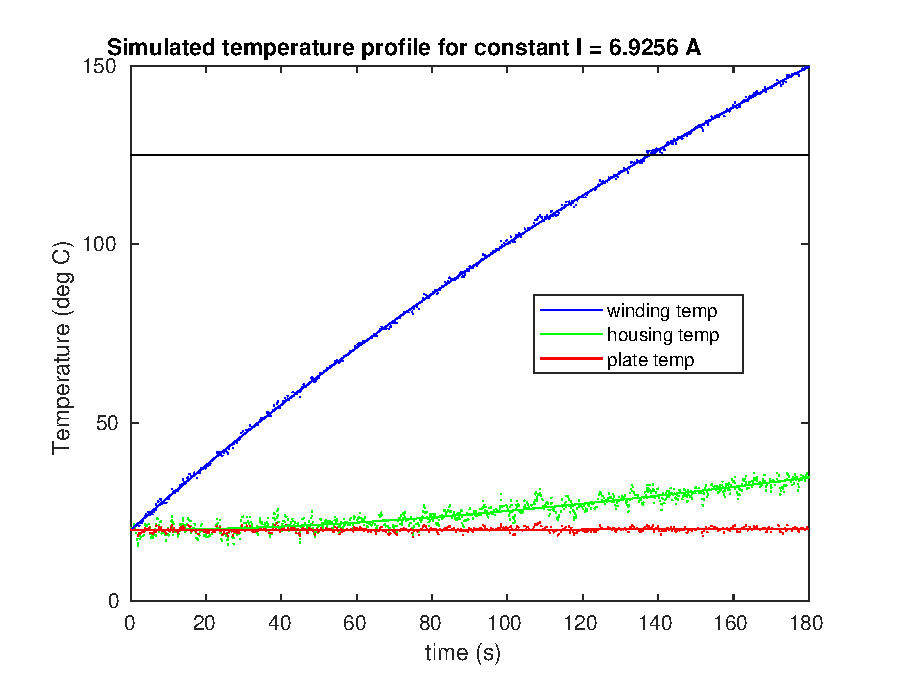
\includegraphics[width=0.7\linewidth]{thermal/Kalman_comparison_standing.eps}
	\caption{Simulated Kalman filter performance during a standing task}
	\label{fig:Kalman_sim_standing}
\end{figure}

\begin{figure}[H]
	\centering
	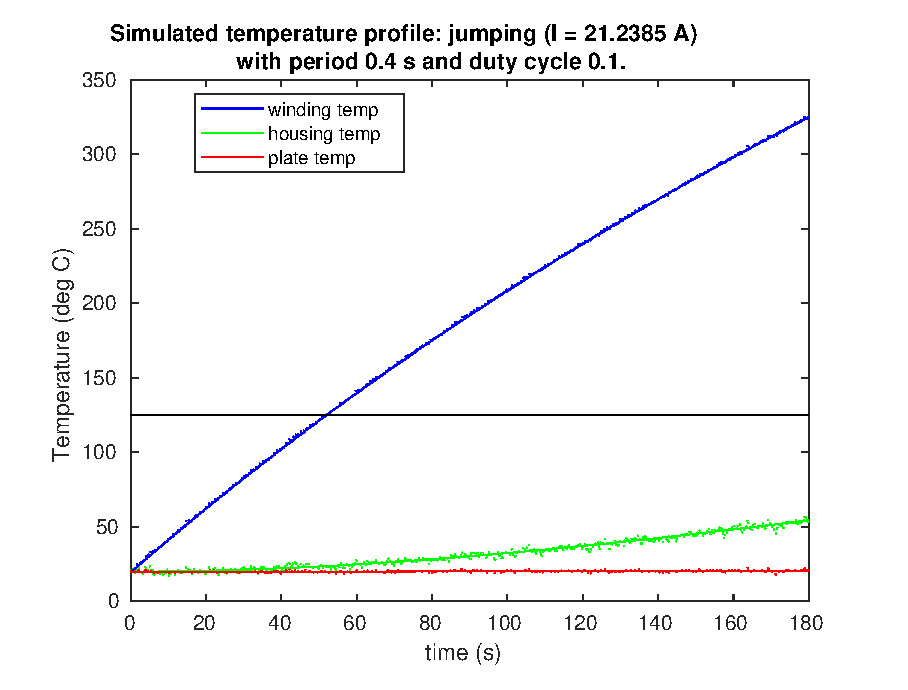
\includegraphics[width=0.7\linewidth]{thermal/Kalman_comparison_jumping.eps}
	\caption{Simulated Kalman filter performance during a jumping task}
	\label{fig:Kalman_sim_jumping}
\end{figure}

\begin{figure}[H]
	\centering
	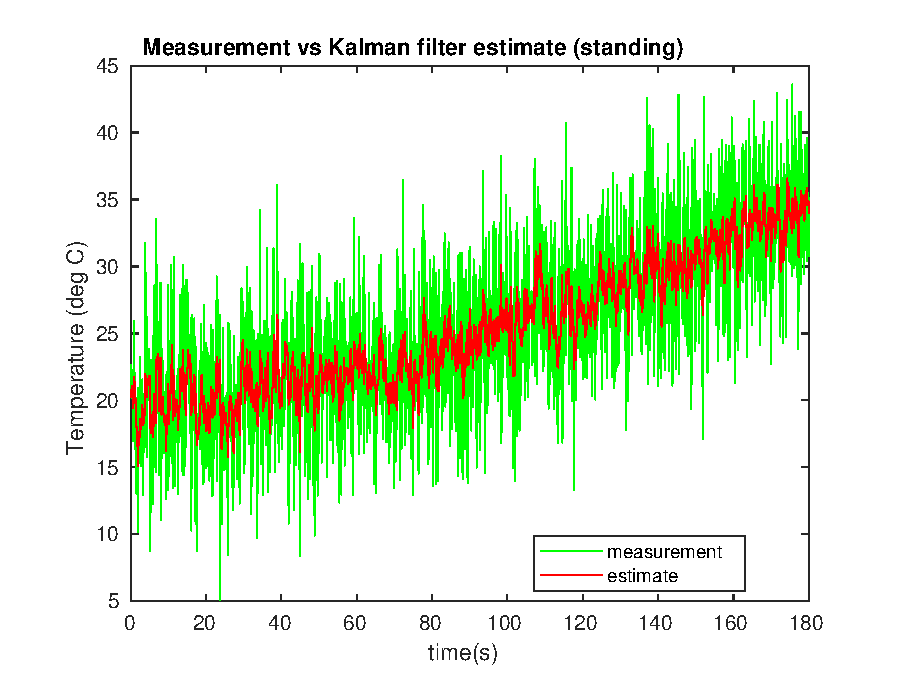
\includegraphics[width=0.7\linewidth]{thermal/Kalman_vs_meas_standing.eps}
	\caption{Comparison of Kalman filter estimate of $T_h$ to noisy measurement of $T_h$ during a standing task}
	\label{fig:meas_vs_Kalman_est_standing}
\end{figure}

\begin{figure}[H]
	\centering
	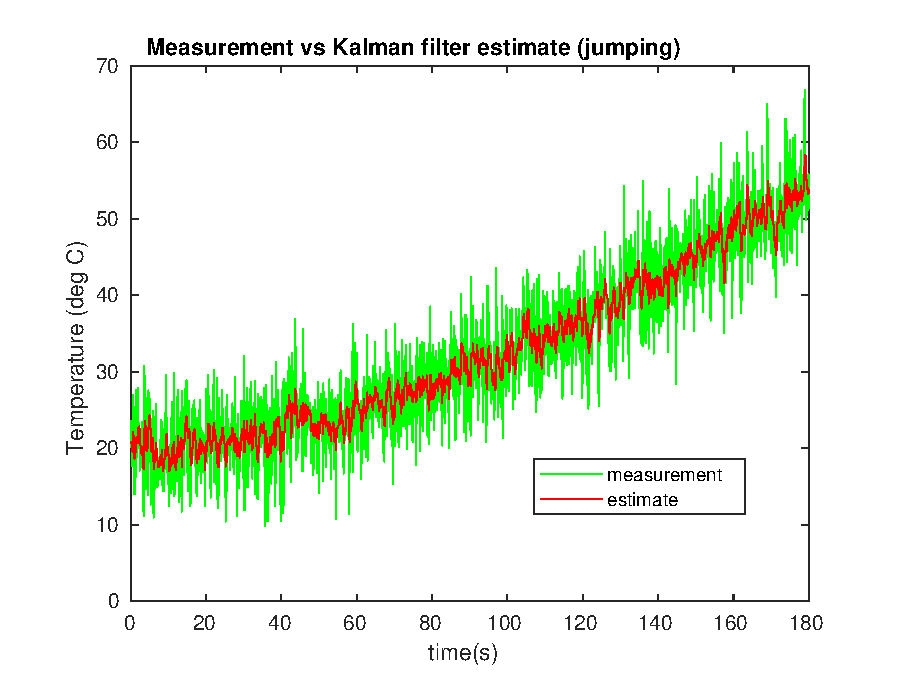
\includegraphics[width=0.7\linewidth]{thermal/Kalman_vs_meas_jumping.eps}
	\caption{Comparison of Kalman filter estimate of $T_h$ to noisy measurement of $T_h$ during a jumping task}
	\label{fig:meas_vs_Kalman_est_jumping}
\end{figure}

\section[Transmission design and analysis]{Transmission design and analysis}
\subsection[Belt selection]{Belt selection}
See``Belts'' document for more detailed analysis and walk-through with links to the proper diagrams.

Assume 4 Nm of torque and 300 rpm needed for the big pulley, with a safety factor of 2 and gearing ratio of 1.5. This means a torque of 2.7 Nm and 450 rpm. Therefore design for 8 Nm (4 Nm * FOS=2) and 450 rpm. Chose the GT2/3 series because we are willing to pay up for the extra strength. Based on charts provided by SDP/SI, we need a 5mm GT3 or 5mm HDT. Using their online calculator and product catalog, we selected a center distance of 140 mm and 98 tooth belt, and 32/48 teeth on the pulleys. This means the small pulley gets a 14.4 Nm torque rating, a length ratio of .92, a width ratio of .6, which means an adjusted torque rating of 7.95, which is close enough to a FOS of 2. Finally, using their calculators, we have sufficient teeth engagement (15 and 25), which is much more than required. The tension should be $18 \text{lbf}\times\text{FOS} (= 2) = 36 \text{lbf}$.

\subsection[Shaft load calculations]{Shaft load calculations}
See ``Belts'' document for links to instructional documents with diagrams and step by step instructions.

\begin{figure}[H]
	\centering
	\includegraphics[width=0.8\linewidth]{beltvector.png}
	\caption{Belt pull vector diagram}
	\label{fig:beltvectors}
\end{figure}

\subsubsection[Tensions and resulting forces]{Tensions and resulting forces}
Figure~\ref{fig:beltvectors} illustrates the tensions in our belt drive. For a torque of 8 Nm = 71 lbf-in.\ with pitch diameters ($P_d$) of $\sim2$ in.\ and $\sim3$ in.\ for driving and driven pulleys respectively, we get four tensions. We then add 36 lbf to each one because we are using the belt as a registration drive:

\begin{subequations}
\begin{equation}
T_{t,driving} = 2.5\times \frac{71}{2} = 88.75\text{ lbf} + 36\text{ lbf} = 124.75\text{ lbf,}
\end{equation}
\begin{equation}
T_{s,driving}= 0.5\times \frac{71}{2} = 17.75\text{ lbf} + 36\text{ lbf} = 53.75\text{ lbf,}
\end{equation}
\begin{equation}
T_{t,driven} = 2.5\times \frac{71}{3} = 59.16\text{ lbf} + 36\text{ lbf} = 95.16\text{ lbf, and}
\end{equation}
\begin{equation}
T_{s,driven} = 0.5\times \frac{71}{3} = 11.83\text{ lbf} + 36\text{ lbf} = 47.83\text{ lbf.}
\end{equation}
\end{subequations}

We then calculate the vector sum correction factor by comparing the center-to-center distance (144 mm or 5.7 in.) of the pulleys to the difference in pitch diameter (3 and 2 inches). The equation is $\frac{D-d}{c} = \frac{3-2}{5.7} = 0.18$ which, from Figure~\ref{fig:vectorsum_correctionfactor}, correlates to a vector sum correction factor of approximately 0.99.

\begin{figure}[H]
	\centering
	\includegraphics[width=0.7\linewidth]{vectorsum_correctionfactor.png}
	\caption{Vector sum correction factor}
	\label{fig:vectorsum_correctionfactor}
\end{figure}

We then add the two force vectors together to get the total force on the shaft and multiply by the vector sum factor. This gives us a driving force of $(124.75+53.75)\times0.99 = 176.7$ lbf and a driven force of $(95.16+47.83)\times0.99 = 141.6$ lbf. These are the forces on each shaft applied at the pulley axially.

If the bearings are equally spaced on the outsides of the pulleys, then the radial force on the bearings are simply $\frac{1}{2}$ the load. If they are both on one side of the pulley in a cantilever, the forces are amplified.

\subsection[Shaft failure calculations]{Shaft failure calculations}

The shafts in the upper part of the robot were expected to transmit 4 Nm of torque to the legs for jumping. The belt and pulley system was designed for this load case according to SDP/SI's recommendations. For our specific torque requirement, considered as $\tau = 8$ Nm in each shaft for a minimum safety factor of 2, and required belt tension $F_{belt\ tension} = 36$ lbf (160 N), the calculated radial force $F_{radial\ equiv}$ due to appropriate belt tension and transmitted torque on the driving (P101) and driven (P103)  shafts are 353 N and 264 N, respectively. Due to the higher effective force of 353 N, shaft P101 (directly coupled to the motors and the small pulleys) are considered most critical. The three remaining shafts are under lighter loads, and therefore should be considered safe if designed similarly to the top shafts.

Given these loads and the geometry of the design, the bearing reaction forces and shaft moments were calculated. The following calculations summarize the key steps of computing the Goodman's line safety factor for the most critical shaft (P101).

\begin{equation}
F_{torque\ equiv} = \frac{\tau}{r_{pulley}} = \frac{8\text{ Nm}}{25.4\text{ mm}} = 315\text{ N,}
\end{equation}

\begin{equation}
F_{radial\ equiv} = \sqrt{F_{belt\ tension}^2 + F_{torque\ equiv}^2} = 353\text{ N.}
\end{equation}

Given maximum shaft bending moment $M_{max}$ of 5.22 Nm (due to the bearing's reaction force) and a shaft diameter $d = 12$ mm, the maximum bending stress is
\begin{equation}
\sigma_{max} = \frac{32 M_{max}}{\pi d^3} = 30.8\text{ MPa,}
\end{equation}
and given a stress concentration factor $K_f = 1.26$, the bending stress amplitude is $\sigma_{ba} = K_f \sigma_{max} = 38.8$ MPa.

For a torque $\tau =  8$ Nm, the shear stress amplitude is
\begin{equation}
\tau_a = \frac{16\tau}{\pi d^3} = 23.6 \text{ MPa,}
\end{equation}

and the Von Mises stress is

\begin{equation}
\sigma_a^{'} = \sqrt{\sigma_{ba}^2 + 3\tau_a^2} = 56.4\text{ MPa.}
\end{equation}

To determine the safety factor, we first calculate the endurance limit $S_e$ given an ultimate tensile strength $S_{ut} = 310$ MPa:

\begin{equation}
S_e = \text{Correction Factor}\times 0.5\times S_{ut} = 0.772\times 0.5\times 310\text{ MPa} = 119.7\text{ MPa}.
\end{equation}

Finally, the safety factor is
\begin{equation}
n_s = \frac{S_e}{\sigma_a^{'}} = 2.12.
\end{equation}

This conservative analysis shows that even for twice our expected operating torque, the Goodman's line safety factor is still 2.  We means that we can expect to be able to run these shafts at about 16 Nm (about 4 times beyond our expected operating region) before failure.

\subsection[Hard stops]{Hard stops}
To implement hard stops on the legs, we opted for a simple design of a bolt and nut. This allowed for easy replacement of the stops, should there be wear or failure. We assumed a worse case scenario of a 4 Nm torque being applied on a leg. We then designed the hard stops to be  1.5 inches (0.0381 m) away from the center of the output shafts. By dividing the torque by the radius, we get a force of 105 N.

Next, we calculate the moment $I$ of the hard stops, approximating them as cylindrical bars, so that

\begin{equation}
I = \frac{1}{3}m(3r^2 + L^2).
\end{equation}

The impact on the bolt is 1.3 inches away from the front face of the robot, so $L = 1.3$ inches. After a few iterations, we ended up selecting a bolt size of $\frac{5}{16}$'', so $r = 0.15625$ inches. From the length $L$ and radius $r$, the volume is $1.63\times 10^{-6} \text{ m}^3$, and given a density (steel) of $\rho = 7800 \text{ kg}/{m}^3$, the bolt has mass $m = 0.0127\text{ kg}$, so from the moment equation above, $I = 0.0075 \text{ kg}\cdot\text{m}^3$.

To calculate the mass stress in the system, we start with the bending moment $I_b$, which is 23.6 lbf (105 N from before) times the length (1.3 inches), or 30.68 in$\cdot$lbf. The centroidal distance is simply the radius of the bolt ($r = 0.15625$ in). The moment of inertia $I_c$ can then be calculated: $I_c = \frac{\pi r^4}{4} = 4.7\times 10^{-4}\text{ in}^4$.

The maximum bending stress is
\begin{equation}
\sigma = I_b\frac{r}{I_c} = 10.24\text{ ksi}.
\end{equation}
A grade 8 steel bolt has a tensile strength of 150 ksi, so the hard stops have a safety factor of almost 15. Although these bolts are suitable as hard stops, they are evidently excessive and can be reduced in size; for example, switching to 10-24 bolts, used throughout the robot, results on a safety factor of 3.3.

\subsection[Link FEA]{Link FEA}
Finite element analysis (FEA) was performed on several waterjetted 6061 aluminum ($2.76\times 10^{8} \text{ N}/\text{m}^2$ yield strength) parts of the robot. For all analyses, the load case was a 250 N force directed into the bottom of the foot. This load approximates a 5g impact force.

\subsubsection[Left and right upper legs]{Left and right upper legs}
\textbf{Load case 1:}
\begin{itemize}
\item \textit{Assumption 1}: Assume half of the load goes into the two side legs equally, with none in the middle leg.
\item \textit{Assumption 2}: Assume a worst case scenario where the load goes in perpendicular to the centerlines.
\end{itemize}
See ``Force calculations for legs'' document for geometry and math for loads. This results in a load of 163 N, and the link passes with a safety factor close to 10. See Figure~\ref{fig:legA_FEA_loadcase1}.

\begin{figure}[H]
\centering
\includegraphics[width=0.8\linewidth]{legA_FEA_loadcase1.png}
\caption[Load case 1 for leg A]{Load case 1 for leg A}
\label{fig:legA_FEA_loadcase1}
\end{figure}

\textbf{Load case 2:}

Using the assumed torque of 4 Nm (from the pulley calculations above) applied at the three holes and the hard stop face locked, we get a safety factor of roughly 10. See Figure~\ref{fig:legA_FEA_loadcase2}. This would not be a shock load, but a load applied after this link is already pressed against the bolt. Given the FOS of 10, failure due to this load case is unlikely.

\begin{figure}[H]
\centering
\includegraphics[width=0.8\linewidth]{legA_FEA_loadcase2.png}
\caption[Load case 2 for leg A]{Load case 2 for leg A}
\label{fig:legA_FEA_loadcase2}
\end{figure}

\subsubsection[Middle upper leg]{Middle upper leg}
\textbf{Load case 3:}

\begin{itemize}
\item \textit{Assumption 1}: Assume all the load goes into only the center portion of the legs
\item \textit{Assumption 2}: Assume similar geometry to previous load case, i.e.\ a load of 325 N tangent to the centerlines.
\end{itemize}
Locked the three holes to simulate a stalled motor. The link passes this simulation with a safety factor of about 1.5. See Figure~\ref{fig:legC_FEA_loadcase3}.

\begin{figure}[H]
\centering
\includegraphics[width=0.8\linewidth]{legC_FEA_loadcase3.png}
\caption[Load case 3 for leg C]{Load case 3 for leg C}
\label{fig:legC_FEA_loadcase3}
\end{figure}

\subsubsection[Support plate]{Support plate}
\textbf{Load case 4:}
Using the loads found in the ``Belts'' document in ideal loading, the support plate will have a FOS of ~49. Given this FOS, the plate can withstand most un-ideal load cases.

\begin{figure}[H]
\centering
\includegraphics[width=0.8\linewidth]{supportplate_FEA_loadcase4.png}
\caption[Load case 4 for the support plate]{Load case 4 for the support plate}
\label{fig:supportplate_FEA_loadcase1}
\end{figure}

\section[Boom selection]{Boom selection}
Recall from Section~\ref{specs:boom}, the initial critical specifications for the choice of boom material and cross section were:
\begin{itemize}
	\item the boom must be 1.2 - 1.5 m long. This is based on the radius of the circular arc to travel from corner to corner in the existing testbed.
	\item the boom must not deflect more than 0.5\% of its length when holding the robot at rest. Assuming the maximum boom length and the maximum 5 kg mass of the robot, the boom must not deflect more than 7.5 mm for with a 50 N load on its end. Deflection in the boom can be modeled as a spring-type dynamic component - thus large boom deflections would further complicate the challenging dynamics of the full system.
	\item the boom mass should be less than 10\% of the robot's mass. Again assuming the maximum robot mass, this limits the boom's mass to 500 g. This ensures that the boom's mass and inertia are negligible compared to those of the robot.
\end{itemize}

This analysis was performed by modeling the boom as a cantilevered Bernoulli-Euler beam with a concentrated load $P$ at its free end. From Bernoulli-Euler tables, the maximum deflection $\delta$ for a beam of length $L$, moment of inertia $I$, and modulus of elasticity $E$ is
\begin{equation}
\delta = \frac{PL^3}{3EI}\text{.}
\end{equation}

It is clear that for a given material, increasing the moment of inertia $I$ decreases the deflection, but often at the cost of increased mass. This was the key tradeoff in this analysis.
We analyzed booms of different common materials (steel, aluminum, and carbon fiber) and different simple cross sections (hollow square and tube). Due to its high strength to weight ratio, we chose a carbon fiber tube, with dimensions $D = 1 \frac{5}{16}$'' (OD) and $d = 1 \frac{3}{16}$'' (ID).  The following calculations show the deflection $\delta$ and mass $m$ of a length $L = 1.5$ m boom supporting a 5 kg robot:
\begin{subequations}
\begin{equation}
P = 5 \text{ kg} \times 9.81\ \frac{\text{m}}{\text{s}^2} = 49 \text{ N,}
\end{equation}
\begin{equation}
I = \frac{\pi\left(D^{4} - d^{4}\right)}{64} = 1.99\times 10^{-8} \text{ m}^4\text{ ,}
\end{equation}
\begin{equation}
\delta = \frac{PL^3}{3EI} = 12.1\text{ mm,}
\end{equation}
\begin{equation}
m = \rho V = \rho A L = \rho \frac{\pi}{4}(D^2 - d^2)L = 0.476\text{ kg,}
\end{equation}
\end{subequations}
where, for carbon fiber, $E = 228 \text{ GPa}$ and $\rho = 2000\  \frac{\text{kg}}{\text{m}^3}$.

Though even this choice of boom does not meet the deflection specification in the worst case length and load scenario, this selection was deemed acceptable by the team and its sponsor, as the calculated deflection is still 0.8\% of the total length.

\section[Counterweight design]{Counterweight design}
The boom counterweight system needed to be able to counter the weight of the boom at the minimum and incrementally counter additional loads up to the entire weight of system (boom and robot combined). The counterweight system needed to be designed with the following important considerations in mind:
\begin{itemize}
\item Counterweight adjustments are incremental with a variety of resolution scales so that the counterweight can be adjusted with precision
\item Counterweight system should be as compact as possible and allow for maximum clearance underneath its pivot so that it does not limit the height to which the robot can jump
\item Counterweight system should be easily adjustable so that iterations of weighting schemes can be quickly tested and adjusted as necessary
\item Counter weight system should have clamping mechanisms built in so that the weights do not oscillate during jumping and cause vibrational inaccuracies in collected data
\end{itemize}

The calculation involved was a simple balancing of moments about the fulcrum point, where

\begin{equation}
M(x) = F\times x
\end{equation}

The moment $M(x)$ at a given location $x$ away from the fulcrum is dependent on the load $F$ at that location. A simplifying assumption that was made was to consider distributed loads such as the weight of the boom to be acting as a point load at a distance halfway between the beginning and end of the load. The resulting free body diagram and calculated loads for the extremes of the required load conditions are shown in Figure~\ref{fig:counterweight}.

\begin{figure}[H]
\centering
\includegraphics[width=0.8\linewidth]{counterweight.png}
\caption[Free body diagram used for designing counterweight system]{Free body diagram used for designing counterweight system}
\label{fig:counterweight}
\end{figure}

From these calculations, we designed and built a counterweight system that was able to handle plate weights ranging from 0.5 kg to 10 kg as well as precision adjustment scale weights ranging from 5 g to 50 g. We purchased three precision weight sets and one plate weight set so that we are able to adjust in a range of 0 to 40 kg with up to 5 g precision.

\chapter[Design Evolution]{Design Evolution}
\section[Mechanical]{Mechanical}
At the Midterm presentation in Winter Quarter, we had a vague idea of what the robot would look like and how it would function (see Figure~ \ref{fig:systemrender_WM}). The purpose of the design at this point was to get the concept of the robot down and discuss the system as a whole. Since then, every single mechanical component has been redesigned in a significant way.

\begin{figure}[H]
\centering
\includegraphics[width=0.5\linewidth]{./images/SystemRender_wintermidterm.JPG}
\caption[CAD rendering of system design as of Winter quarter midterm]{CAD rendering of system design as of Winter quarter midterm}
\label{fig:systemrender_WM}
\end{figure}

At the Winter Quarter Final, the base and boom holder assemblies were fully designed with the robot incomplete (see Figure~\ref{fig:systemrender_WF}). We had made $\frac{3}{4}$ of the base and boom holder assembly. We have since finished making it, including some minor redesigns of components like the counterweight holder and base block where we switched from two roller bearings to a roller and a thrust bearing.

\begin{figure}[H]
\centering
\includegraphics[width=0.5\linewidth]{./images/systemrender_winterfinal.png}
\caption[CAD rendering of system design as of Winter quarter final]{CAD rendering of system design as of Winter quarter final}
\label{fig:systemrender_WF}
\end{figure}

At the Spring Quarter Midterm, the entire system was designed in a way that was supposed to be final (see Figure~\ref{fig:systemrender_SM}). We had finished the construction of the entire base and boom holder assembly with the exception of the counterweight system. We had the entire robot manufactured and assembled as well, but we have since redesigned many of those components such as changing from L brackets to square tubing for the legs.

\begin{figure}[H]
\centering
\includegraphics[width=0.5\linewidth]{./images/systemrender_springmidterm.JPG}
\caption[CAD rendering of system design as of Spring quarter midterm]{CAD rendering of system design as of Spring quarter midterm}
\label{fig:systemrender_SM}
\end{figure}

\section[Electrical]{Electrical}
The layout of the electrical system took shape quickly during the start of winter quarter, when we decided to use a CAN bus and determined that our nodes would be a single-board computer, three motor control boards, three boom encoder boards, and one board for communicating with the IMU and the force sensor. As we went through the motor selection process, we also decided to use the Copley Accelus motor controller panels to control our motors. By the end of winter quarter, we had designed and ordered the first versions of each of the custom Tiva boards and were set on the Copley amplifiers.

At the start of spring quarter, we went through two quick iterations of our custom Tiva boards to fix circuit bugs and make sure that we had the exact functionality we wanted out of the boards. Overall, there were no significant additions or subtractions from the design of the custom boards. We also decided to use a set of four 12 V batteries in series to power our motors and the Copley amplifiers, and had to design the power electronics to make sure that the system was still safe.

From the midterm of Spring quarter to the end of Spring quarter, no major changes were made to the electrical design. The only additions were a second switch in the positive voltage line of the battery bank, as an additional safety precaution. At the end of spring quarter, all of the pieces of the electrical system were assembled and functioning as intended. 


\section[Software]{Software}
Over the course of both quarters, there was roughly linear progress in terms of building the necessary software for our robot. As the mechanical design came further and further along, we introduced new functionality into the firmware of the Tiva boards and developed the CAN bus message hierarchy used by the Tiva boards and the Raspberry Pi. At the end of Spring quarter, we had high-functioning firmware for each Tiva board and could send and receive messages to and from the Raspberry Pi.

As Tiva firmware development progressed, we simultaneously developed a multi-threaded real-time control program on the Raspberry Pi, with separate threads for reading the CAN bus, calculating control inputs and writing them to the CAN bus, and streaming operational data back to the client program over UART.

\chapter[Final Design Description]{Final Design Description}
\section[Mechanical]{Mechanical}
The system, shown in Figure~\ref{fig:systemrender_SF}, is separated into two primary systems, the robot and the holder, each with their own subsystems.

\begin{figure}[H]
\centering
\includegraphics[width=0.5\linewidth]{./images/systemrender_springfinal.JPG}
\caption[CAD rendering of system design as of Spring quarter final]{CAD rendering of system design as of Spring quarter final}
\label{fig:systemrender_SF}
\end{figure}

\subsection[Robot]{Robot}
The robot contains three subsystems: the body, the legs and the foot.
\subsubsection[Body]{Body}
The robot body's primary function is to hold all the components which transfer the energy from the motors to the legs. It also houses electronics including the leg encoders and the IMU. Finally, it connects to the boom assembly through the roll bearing housing.
\subsubsection[Legs]{Legs}
The robot legs' primary function is to support the weight of the robot while transferring the rotation of the shafts into linear motion, allowing jumping and balancing. The lengths of the legs were carefully selected through an optimization program to allow for the most power and motion, while needed the least power.
\subsubsection[Foot]{Foot}
The robot foot's primary functions are to hold the bumper and force sensor. The foot system allows for a softer landing and easier control through the use of a round rubber bumper. The foot system also passes the majority of the in axis force from the jumping through the force sensor, allowing for a rough tracking and collection of forces. The force sensor will eventually be replaced by a much nicer one currently on the old single axis system, so the foot system is only a temporary solution and will be redesigned.

\subsection[Holder]{Holder}
The holder contains three subsystems: the boom, the base, and the counterweight.
\subsubsection[Boom]{Boom}
The boom's primary function is to connect the robot with the base in the lightest way possible. Carbon fiber is used due to its high strength to weight ratio.
\subsubsection[Base]{Base}
The base's primary function is to allow for the movement of the robot and boom in a controlled manner with the option of locking any of the 3 axis (roll, pitch, and yaw).
\subsubsection[Counterweight]{Counterweight}
The counterweight's primary function is to offset the weight of the boom, with the option of adding more weight to simulate different gravities. The design allows for both fine and coarse adjustment through the addition of both small and large weights.

\section[Electrical]{Electrical}
Parts of the electrical system are on the robot itself, on the base of the boom, and separate from the mechanical system entirely. On the robot, there are three motor control Tiva boards, one of the boom encoder Tiva boards (to capture the roll of the robot relative to the boom), and the Tiva board for the force sensor and IMU. At the base of the boom, there are two more of the boom encoder Tiva boards, to capture the pitch and yaw of the boom. Away from the base of the boom, there is a Raspberry Pi, which runs the main controller, as well as the three Copley Accelus motor drivers, the bank of 12 V batteries, and the power switches for the 48 V and 5 V supplies. The CAN bus runs from the Raspberry Pi to the base of the boom and out along the boom to the other group of boards, along with +5 V power, ground, and PWM signals for the Copley amplifiers. Cables for hall signals and motor phases also run along the boom between each motor and its corresponding amplifier.

Each of the custom Tiva boards uses a TM4C123G microcontroller and serves as a node on the CAN bus of the robot. The three boom encoder boards communicate over SPI with AEAT-6600 magnetic encoders to track the angles of the three degrees of freedom of the boom, and then report the angles back over the CAN bus to the Raspberry Pi. In a similar manner, the board for the IMU and force sensor communicates over I2C with the IMU and reads an analog signal from the force sensor, and then reports the data back over the CAN bus. The three motor control boards communicate over SPI with RLS Orbis magnetic encoders to track the positions of the output shafts for each of the three motors. Each board also sends a PWM signal to the one of the Copley amplifiers that controls the current that the the Copley tries to put through the motor. The boards can use the PWM output to the Copley amplifiers to close a position control loop using reference positions received from the Raspberry Pi over the CAN bus and the encoder signals, or enter a current control mode based on commanded currents which are also received from the Raspberry Pi over the CAN bus. 

The Tiva boards and the Raspberry Pi are powered from a 5 V, 10 A wall supply. The only switch in the 5 V power line is a small barrel jack. The Copley amplifiers, and thus the motors, are powered from a group of 4 $\times$ 12 V, 35 Ah batteries that are wired in series. There is one large switch in the +48 V power line, as well as an 80 A circuit breaker, which acts as a second switch. In accordance with the Copley amplifier datasheet, there are fuses on the power input and two of the three motor phase outputs. In the current configuration, these fuses are all 35 A fuses, which would protect the amplifiers in the case of a short but are well above the stall current of the motors.

\section[Software]{Software}
The firmware on the robot is an example of distributed hierarchical control. A high-level task space controller runs at 500 Hz in one thread of the main program, \texttt{main.c} on the Raspberry Pi, and it sends commands to lower-level torque/position controllers running at 1 kHz on the motor control Tivas.
\subsection[Raspberry Pi firmware]{Raspberry Pi firmware}\label{sec:PiFirmware}
The main program on the Raspberry Pi, \texttt{main.c}, uses a number of libraries, including
\begin{itemize}
\item \texttt{pthreads}\footnote{\url{http://man7.org/linux/man-pages/man7/pthreads.7.html}} for multithreading,
\item SocketCAN\footnote{\url{https://www.kernel.org/doc/Documentation/networking/can.txt}} for interfacing with the CAN bus,
\item GNU Scientific Library\footnote{\url{https://www.gnu.org/software/gsl/}} (GSL) for matrix math and interpolation, and
\item WiringPi\footnote{\url{http://wiringpi.com/}} to make the Pi's GPIO pins accessible to userspace programs like \texttt{main.c}.
\end{itemize}

The motivation for making \texttt{main.c} a multithreading program is to separate timing-critical control computations from slower and less crucial tasks like communicating with the client via UART. These threads share a circular buffer; the control thread puts data in the buffer and the UART thread reads data from the buffer.

Should computation speed become a limiting factor, we recommend replacing GSL with Automatically-Tuned Linear Algebra Software\footnote{\url{http://math-atlas.sourceforge.net/}} (ATLAS), which has already been set up on the Pi. Building ATLAS on the Pi required us to disable CPU throttling, effectively overclocking the Pi: by default, it runs at 700 MHz; we are running it at \textit{1.2 GHz}, so it is essential to actively cool the Pi.

\subsection[Tiva firmware]{Tiva firmware}
Each Tiva program resembles a simplified version of the Pi's \texttt{main.c}. The firmware is built on Texas Instruments' \texttt{Tivaware}\footnote{\url{http://www.ti.com/tool/SW-TM4C}} driver library.
\subsubsection[Motor control firmware]{Motor control firmware}
The motor control firmware is built around a 1 kHz timer-driven interrupt. An asynchronous process reads from the CAN bus and stores received commands (either position or current references)in a global variable. The interrupt service routine (ISR) checks the global variable, reads from a RLS Orbis encoder over SPI, and calculates a current required to track the reference signal. This current command is sent to the appropriate Copley Accelus amplifier via a 25 kHz PWM signal.
\subsubsection[Boom encoder firmware]{Boom encoder firmware}
Like the motor control firmware, the boom encoder firmware is also built around a timer-driven interrupt, currently set to 10 Hz. The ISR reads from an AEAT-6600 encoder over SPI, converts the reading to tenths of a degree, and writes the converted value to the CAN bus. If the robot is using boom angles in any control computations, the boom interrupt frequency will need to increase.
\subsubsection[IMU and force sensor firmware]{IMU and force sensor firmware}
The firmware for the IMU and force sensor Tiva is also built around a timer-driven interrupt, currently set to 100 Hz. The ISR reads from an analog-output force sensor and (for now) from a STM LSM6DS33 IMU over I2C. The ISR then writes the measured force and accelerations to the CAN bus. If the robot is using these values in any control computations, this interrupt frequency will also need to be increase.

\subsection[Client]{Client}
The client program is very minimal, with the understanding that the end user's research tasks will dictate most of the structure of the client. At present, the client provides a serial interface with the Raspberry Pi and some basic plotting functions to visualize data received from the Pi.

\chapter[Testing Procedures and Performance Results]{Testing Procedures and Performance Results}
By the end of the winter quarter, it was evident to the team and the instructors that high level control of the robot before the spring final was a very ambitious task.  Instead we shifted our focus to developing the robust low level functionality that would be required to build up the desired high level behavior in the future.  At this point, the primary goal for the end of spring quarter was to do an open loop jump to demonstrate the potential of the robot in the future upon development of high level controllers.

Before going straight to a jump, we wanted to validate our kinematic models and motor selection by finding the current required in the motors to support the robot's full 5 kg weight. This requires a 50 N force at the foot, mapping through the actuator Jacobian to about 1.5 Nm in each of the two outside legs.  Due to the 1.5:1 pulley ratio between the legs and the motors, this means we expected the outside two motors to supply 1 Nm of torque, corresponding to 4.6 A.  

We tested this by putting the robot in position hold mode, commanding a fairly “extended” leg position, setting the full weight of the robot on the leg, and reading the current flowing through the windings.  In this setup, the outside motors required between 4.0 - 5.0 A, verifying our expected torque requirements.

Once we were confident in our kinematic model and our motor selection, we began our first attempts at a feed-forward jump by commanding a current impulse to the two outside motors. We began in position hold mode in a “squatted” position, then switching to current control mode, increasing the command magnitude and duration conservatively until a satisfactory jump was achieved. Ultimately, when reaching an command of 19 A over 0.15 s, we decided that this was the maximum power we were comfortable providing at this point without any additional control or safeties. Nonetheless, as shown in Figure~\ref{fig:jumpfreezeframe}, slow motion video footage of one of these jumps shows a maximum jump height of about 3.5 inches (9 cm), narrowly missing our target of 10 cm.

\begin{figure}[H]
\centering
\includegraphics[width=0.5\linewidth]{./images/jumpfreezeframe.png}
\caption[Still frame showing maximum height (9 cm) achieved in an open-loop jump]{Still frame showing maximum height (9 cm) achieved in an open-loop jump}
\label{fig:jumpfreezeframe}
\end{figure}

The team is optimistic about this result for several reasons. First, our feedforward current impulses are perhaps the least controlled and most unintelligent way to achieve a jump. The actuator Jacobian that maps the actuated joint torques to wrenches at the foot is configuration dependent, and therefore it is difficult to predict and control the jump and the applied forces without any kind of control strategy. 

Second, our jumps were done using only the two outside motors - the center motor was powered off during the jump tests. While it is convenient to think of this center motor as only controlling the angle of the foot while the two outside motors provide the power for the jump, this is an oversimplification - utilizing the center motor would surely add to the jump height.

Even a simple controller for this motor would greatly help the jump, as we noticed that some of the motors' power went towards a small component of horizontal velocity, rather than all towards the vertical velocity as desired. We think that even a simple position control of this motor to keep the bottom leg vertical while the two outside motors are producing high torque would help keep the leg forces vertical, resulting in a higher jump.

From our kinematic model developed during the first quarter, we had expected to require 12.6 A from each of the two outside motors to achieve a 10 cm jump, but our jumps required 19 A - about a 50\% difference. We cannot definitively account for this discrepancy, but it is likely that the factors above are responsible. It is encouraging that the robot is able to jump using a current within the same order of magnitude as our prediction, but this should be reevaluated once a better jumping strategy is implemented.

\chapter[Suggested Next Steps]{Suggested Next Steps}
The following considerations and next steps must be taken to ensure both the short term and long term success of the design.
\section[Mechanical]{Mechanical}
\subsection[Modified motor shaft/drive shaft coupling]{Modified motor shaft/drive shaft coupling}
As we began increasing the loads on our motors, we found that the Maxon motor shafts would often decouple from the drive shafts. We attribute this failure to our use of set screws to transmit these high torques. Several different levels of modifications should be made to improve this coupling:
\begin{itemize}
\item Add a second set screw: The timing pulleys use two set screws, and we have not yet seen these decouple from the shaft. Perhaps this may be the easy solution.
\item Add flats to the motor shaft: Flats would increase the gripping strength of the set screw.
\item Use a key and keyway: This is the most rigorous mechanical solution, but would require non-trivial modifications to the two coupled shafts.
\end{itemize}
\subsection[Integrate new force sensor]{Integrate new force sensor}
The force sensor currently on our robot is a simple and cheap 1-axis sensor. It can be useful in the short term as a ground detection device, but ultimately it should get replaced by the 6-axis force sensor that is currently on the 1-DOF hopping robot in the NxR lab.

\subsection[Design for assembly]{Design for assembly}
Currently, mechanical assembly is a two-person job and takes about 2 hours to complete. Several DFA considerations could be taken to improve the assembly process, such as designing a jig for belt tensioning.

\subsection[Harness for supporting the robot]{Harness for supporting the robot}
Executing a jump currently is also at least a two person process - one to man the controls and emergency stop, and another (or two) to support the robot and keep it upright. Until the robot is intelligent enough to stand, balance, jump, and land on its own, a harness is required to keep the robot from crashing into the floor. This would allow the robot to be operated by one person only.

\subsection[Patch the carbon fiber tube]{Patch the carbon fiber tube}
An unfortunate accident during assembly resulted in about a 1 inch long crack in the carbon fiber boom. This was patched temporarily with duct tape, but this should be properly repaired with a commercial carbon fiber patch.

\section[Electrical]{Electrical}
\subsection[Future board iterations]{Future board iterations}
Version 4 of each of the custom PCBs will be required for several necessary upgrades and luxury items:
\begin{itemize}
\item Prepare for an upgraded IMU and force sensor
\item Break out additional digital and analog I/O pins, for flexibility in future upgrades
\item Add +5 V and GND connections to the programming headers to streamline the programming process. This would remove the need to power all boards while programming, and gives a convenient location to connect common ground between the custom board and the programming Tiva.
\end{itemize}

\subsection[Robustify cable connectors]{Robustify cable connectors}
Most our cables use either screw terminal blocks or 0.1'' headers to connect and transmit signals. These were convenient for us to use in the short term, but are not the most robust and they have the potential for the user to plug in a cable backwards. It would be nice to use polarizing Molex connectors at these locations.

\subsection[Cooling the Raspberry Pi]{Cooling the Raspberry Pi}
The temporary fan/heatsink assembly on the Raspberry Pi should be replaced with a more professional active cooling system. Better cooling can also be achieved by attaching the Pi's CAN adapter by running wires instead of mounting it directly over the Pi's hot processor.

\section[Software]{Software}
\subsection[Motor control Tiva boards]{Motor control Tiva boards}
\begin{itemize}
\item Implement configuration dependent PID gains for each controller, or a different position controller altogether (such as a task-space pose controller). Due to the closed linkage, it is possible for the motors to fight each other while moving to a position. A controller should be implemented that ensures cooperation between the motors in this mode.
\item Estimate the motor winding temperatures. With our thermal model, this can be estimated with a Kalman filter (see Section~\ref{sec:thermalmodel}).
\end{itemize}

\subsection[Raspberry Pi]{Raspberry Pi}
The software on the Raspberry Pi is primarily used to implement the robot controllers. Short term goals include writing stable controllers for balancing and landing a jump. These are prerequisites for developing more sophisticated controllers required for locomotion on soft ground.

Should computation speed become a limiting factor, we recommend replacing GSL (see Section~\ref{sec:PiFirmware}) with Automatically-Tuned Linear Algebra Software (ATLAS), which has already been set up on the Pi and is available at \url{http://math-atlas.sourceforge.net/}

From Section~\ref{sec:prosconsFK}, we recommend searching or devising a forward kinematics algorithm that is free from the jump discontinuities of \texttt{geomFK} and the unbounded execution time of \texttt{NRFK}.

\subsection[Client]{Client}
\begin{itemize}
\item Full data logging. The user should be able to read any recorded data from a experiment into a high level analysis software like MATLAB.
\item Interface with the dynamic model. As more complex controllers are written, it would be useful to use \texttt{trep}\footnote{\url{http://murpheylab.github.io/trep/}} to validate some behaviors before executing them on the robot.
\item (optional) Add a second serial interface to allow the end user to connect to any of the Tivas' UART modules for debugging, data logging, and visualization.
\item (optional) Interface with Robot Operating System (ROS). This will be easier if the client program is ported to Python.
\end{itemize}

\chapter[Other Documentation]{Other Documentation}
\begin{itemize}
\item Assembly Instructions
\item User Guide
\item Software Documentation
\item Quickstart Instructional Video
\item ``Belts'' calculations
\item ``Shafts'' calculations
\end{itemize}

\bibliography{ref}
\bibliographystyle{plain}

\end{document}